\chapter{Valutazione}
\label{cap:valutazione}

Nei capitoli precedenti il modello di scheduling policy-driven è stato definito formalmente e tradotto in un sistema funzionante in ambiente Kubernetes. Questo capitolo ne presenta la valutazione sperimentale, rivolta al comportamento dinamico del sistema.

% ------------------------------------------------------------ %

\section{Obiettivi della Valutazione}
\label{sec:obiettivi_valutazione}

Le politiche che governano l'assegnazione di un task non sono tutte uguali rispetto al momento in cui vengono valutate. Le politiche statiche, ovvero $c_{prop}$, $c_{geo}$, $c_{static}$ e $c_{auth}$, valutano un task rispetto a proprietà fissate a livello di configurazione, come le caratteristiche dei nodi, la residenza dei dataset o i permessi degli issuer: per un dato task e una data configurazione del cluster, il loro esito è determinato e non cambia nel tempo, dato che il task o soddisfa quei vincoli o non li soddisfa affatto. Invece, la politica di Chinese Wall $c_{wall}$ si comporta in modo diverso, perché il suo esito dipende dalla storia delle esecuzioni sui nodi. La memoria contestuale $\Lambda(n)$ che ciascun nodo accumula cresce a ogni task eseguito e viene azzerata dalla sanificazione, per cui lo stesso task può risultare ammissibile su un nodo in un istante e non ammissibile in un altro. È quindi l'unica politica il cui effetto sull'assegnazione, e in particolare sulla latenza di scheduling, varia con l'evoluzione dello stato del cluster.

È proprio questo a rendere $c_{wall}$ la componente più significativa da valutare sperimentalmente, poiché il suo comportamento non dipende solamente dalla configurazione del sistema, ma emerge osservando il sistema in funzione, dall'interazione tra i task che contaminano i nodi e la sanificazione che li ripulisce. La valutazione si concentra quindi su questa politica, con l'obiettivo di osservarne e misurarne il comportamento.

% ------------------------------------------------------------ %

\subsection{Fattori in Gioco}
\label{subsec:fattori_valutazione}

L'evoluzione della memoria contestuale, e con essa il modo in cui $c_{wall}$ blocca o lascia passare i task nel tempo, è governata da due fattori. Il primo è la densità di conflitto tra i contesti, indicata nel seguito con $\rho$, ovvero la frazione di coppie di contesti dichiarate in conflitto tra loro. Il secondo è la frequenza con cui i nodi vengono sanificati, espressa dall'intervallo di sanificazione periodica e indicata nel seguito con $\tau$, che stabilisce ogni quanto la procedura viene eseguita su ciascun nodo, e quindi per quanto tempo le tracce contestuali di un task rimangono sul nodo prima della pulizia successiva. I due fattori agiscono su aspetti distinti:
\begin{itemize}
    \item la densità di conflitto influisce sulla \emph{probabilità} che un task da assegnare venga bloccato, dato che più coppie sono in conflitto più è facile che un nodo contaminato risulti inammissibile per il task in valutazione;
    \item l'intervallo di sanificazione influisce invece sul \emph{tempo} che un task già bloccato deve attendere prima di poter essere schedulato, dato che il suo sblocco dipende dal successivo ciclo di sanificazione del nodo.
\end{itemize}

La valutazione è perciò organizzata in due esperimenti, ciascuno dei quali isola uno dei due fattori facendolo variare mentre l'altro rimane fisso, così da attribuire gli effetti osservati alla variabile in studio.

% ------------------------------------------------------------ %

\subsection{Perimetro e Aspettative}
\label{subsec:perimetro_valutazione}

Per isolare questo comportamento, la valutazione lascia fuori tutto ciò che non vi contribuisce, a partire dalle politiche statiche già discusse. Un caso a parte è il consumo di risorse dei nodi, anch'esso escluso dagli esperimenti. Difatti, come stabilito tra le assunzioni iniziali, i task sono \emph{black-box}, ovvero unità di calcolo simulate, e negli esperimenti non occupano CPU o memoria in misura tale da saturare i nodi. Questa scelta è coerente con il modello, che non considera la capacità residua dei nodi, dato che in Kubernetes la disponibilità di risorse è già gestita dal plugin nativo \texttt{NodeResourcesFit} dello scheduler~\cite{k8s-scheduler-config}, esterno alle politiche di questa tesi. Negli scenari di valutazione, quindi, un task non viene mai ritardato per insufficienza di risorse, ma soltanto dalle politiche del modello, il che consente di attribuire ogni ritardo osservato a $c_{wall}$. In uno scenario reale la saturazione dei nodi sarebbe un ulteriore fattore di rallentamento, come si discuterà tra le limitazioni conclusive.

Quanto ai risultati attesi, i due esperimenti condividono lo stesso compromesso di fondo tra disponibilità dei nodi e reattività dello scheduling. Ci si attende che la latenza di scheduling cresca con la densità di conflitto $\rho$, perché più coppie in conflitto rendono più probabile che ogni nodo candidato sia contaminato da un contesto incompatibile. Invece, ci si attende un andamento a U rispetto all'intervallo di sanificazione $\tau$: valori troppo piccoli tengono i nodi quasi sempre in sanificazione e quindi indisponibili, valori troppo grandi lasciano le tracce sui nodi troppo a lungo, e tra i due estremi dovrebbe esistere un valore che minimizza la latenza. 

% ------------------------------------------------------------ %

\section{Configurazione Sperimentale}
\label{sec:configurazione_sperimentale}

Gli esperimenti sono stati condotti su un cluster kind con Kubernetes 1.34, composto da un control-plane e 5 nodi worker ospitati sulla stessa macchina. Si tratta della configurazione a cluster singolo già assunta nella Sezione~\ref{impl:cluster_singolo}, con un'unica istanza dello scheduler che assegna i \texttt{Pod} in sequenza. 

% ------------------------------------------------------------ %

\subsection{Cluster ed Entità}
\label{subsec:cluster_entita_valutazione}

I cinque worker sono configurati in modo identico. Condividono la stessa classe di proprietà $\alpha(n)$, ottenuta definendo un'unica proprietà astratta $p \in \mathcal{P}$ con un solo livello oltre a quello di default, ovvero $\mathcal{L}_p = \{0,\, 1\}$, raggiunto da ogni nodo, hanno la stessa località $loc(n)$ in un unico gruppo geografico, e ogni dataset del sistema è disponibile su ciascuno di essi. Questa omogeneità è la riproduzione della situazione in cui $c_{wall}$ opera davvero: un task attraversa prima le politiche statiche, che restringono i candidati ai nodi che soddisfano i suoi vincoli, e su quel sottoinsieme, ormai omogeneo rispetto ai requisiti statici, la sola politica che continua a discriminare tra un nodo e l'altro è $c_{wall}$. Configurare i worker come un pool omogeneo colloca quindi l'esperimento direttamente nel punto della pipeline in cui la politica dinamica agisce. Ne consegue che $c_{prop}$, $c_{geo}$ e $c_{static}$ risultano sempre soddisfatte e che l'indicatore $\phi_{prop}$ assume lo stesso valore su ogni nodo, senza influenzare la scelta finale. Le politiche statiche restano attive e ogni task le attraversa, ma non distinguono tra i nodi, cosicché ogni differenza di latenza tra scenari è attribuibile unicamente a $c_{wall}$. 

Le entità del sistema seguono lo stesso criterio di leggibilità. Sono definiti $K = 10$ contesti e, per ciascuno, un dataset che appartiene a quel solo contesto, non statico e disponibile su tutti i nodi, e un issuer autorizzato esclusivamente su di esso, mentre ogni task richiede il solo dataset del contesto del proprio issuer, così che $c_{auth}$ risulti sempre soddisfatta. Inoltre, poiché ogni dataset è replicato su tutti i nodi, l'indicatore $\phi_{transfer}$ assume lo stesso valore ovunque, senza concorrere a distinguere un nodo da un altro. In questo modo $auth(iss(t))$, $ctx^*(t)$ e la traccia depositata dall'esecuzione coincidono tutti con un unico contesto, e il comportamento di $c_{wall}$ dipende unicamente dalle coppie in conflitto, senza le ambiguità di issuer con più autorizzazioni o task con più dataset.

Essendo quindi uniformi su tutti i nodi sia $\phi_{prop}$ sia $\phi_{transfer}$, la scelta tra i nodi ammissibili ricade, come anticipato nella Sezione~\ref{subsec:scheduler}, sui plugin di \emph{Score} nativi rimasti attivi nella configurazione, che però non incidono direttamente sul blocco dei task, il quale dipende unicamente dalla fase di filtraggio.

Dati $K$ contesti esistono $\binom{K}{2} = \frac{K(K-1)}{2} = 45$ coppie possibili, e il parametro $\rho$ ne è la frazione in conflitto, selezionata fissando una permutazione delle $\binom{K}{2}$ coppie determinata da un \emph{seed} e prendendone le prime $\lceil \rho \binom{K}{2} \rceil$. Ne derivano scenari annidati, in cui l'insieme delle coppie a densità maggiore contiene quello a densità minore, con l'asse dell'esperimento monotono per costruzione, e un grafo dei conflitti dipendente solo dal \emph{seed} e quindi identico tra le repliche di uno stesso scenario. A ogni contesto si associa il suo grado, ovvero il numero di altri contesti con cui è dichiarato in conflitto, il cui valore medio cresce con la densità secondo circa $\rho\,(K-1)$: è questa, più della densità complessiva, la grandezza che determina quanto è probabile che un nodo contaminato risulti inammissibile per un task. L'intervallo di sanificazione $\tau$, l'altro parametro fatto variare negli esperimenti, corrisponde nel prototipo alla sanificazione periodica eseguita dal \emph{node-controller}, la sola strategia tra quelle discusse nella Sezione~\ref{subsec:chinese_wall} a essere stata implementata.

% ------------------------------------------------------------ %

\subsection{Workload e Metriche}
\label{subsec:workload_metriche}

Ogni run sperimentale sottomette $N = 200$ task, ciascuno con un contesto estratto uniformemente tra i $K$ disponibili da un generatore con \emph{seed} fissato, a un rate costante di un task al secondo, e ogni task ha una durata simulata di 20 secondi. Il rate costante è una scelta necessaria, dato che una sottomissione in burst misurerebbe soprattutto la contesa sull'API server di Kubernetes, mentre inviare un task solo dopo il completamento del precedente terrebbe sui nodi un task per volta, senza mai far coesistere task di contesti diversi. Soltanto un flusso regolare mantiene più task attivi insieme facendo crescere la memoria contestuale dei nodi nelle stesse condizioni a ogni ripetizione. Anche il numero di task è importante, perché una run deve durare abbastanza da coprire più cicli di sanificazione anche per il valore di $\tau$ più grande della griglia; con una run troppo breve, a quei valori la sanificazione scatterebbe appena una o due volte, e la misura non rifletterebbe il suo reale effetto.

Ogni scenario è ripetuto in 5 repliche con \emph{seed} accoppiati, dove la replica di indice $r$ rigioca la stessa sequenza di task in tutti gli scenari, così che il confronto sia appaiato, mentre repliche diverse usano sequenze diverse. Le curve dei valori medi nelle seguenti figure riportano la media tra repliche con una banda pari a una deviazione standard tra di esse, che misura la ripetibilità dell'esperimento e non la dispersione dei task all'interno di una run.

Le metriche raccolte descrivono il fenomeno da più punti di vista. La misura principale è la latenza di scheduling, il tempo tra la sottomissione della richiesta e il binding del \texttt{Pod} a un nodo, riferita al singolo task. La accompagnano la frazione di task bloccati, cioè respinti almeno una volta dallo scheduler prima di essere assegnati, e la causa del blocco, che distingue i task esclusi soltanto perché il nodo era in sanificazione da quelli che, nel corso dell'attesa, hanno incontrato anche una traccia in conflitto. Per i soli task bloccati si misura l'attesa, dal primo rifiuto al binding, mentre dal lato dei nodi si misura l'indisponibilità, come frazione del tempo in cui un nodo è fuori da $\mathcal{N}$ perché in sanificazione. Il makespan, dal primo invio all'ultimo completamento, offre infine una vista sull'intero carico anziché sul singolo task, e la distribuzione cumulata della latenza affianca la media per mostrare come i task si dividano tra quelli schedulati quasi subito e quelli costretti a una lunga attesa, una separazione che la media da sola nasconde.

Infine, tra una run sperimentale e la successiva, il cluster viene riportato a uno stato noto, rimuovendo richieste, \texttt{Job} e \texttt{Pod} residui e azzerando memoria contestuale e \emph{taint} di sanificazione su ogni nodo, così che nessuna run risenta della precedente.

La Tabella~\ref{tab:parametri_valutazione} riassume la configurazione di entrambi gli esperimenti. I parametri della prima parte sono comuni, mentre la seconda riporta, per ciascun esperimento, il valore tenuto fisso e la griglia di valori assunti dalla variabile da valutare.

\begin{table}[ht]
    \centering
    \begin{tabular}{ll}
        \toprule
        \textbf{Parametro} & \textbf{Valore} \\
        \midrule
        Nodi worker & 5 \\
        Contesti $K$ & 10 \\
        Task per run $N$ & 200 \\
        Rate di sottomissione & 1 task al secondo \\
        Durata di un task & 20 secondi \\
        Repliche per scenario & 5 \\
        \midrule
        \multicolumn{2}{l}{\textit{Impatto dei conflitti (Sezione~\ref{sec:impatto_conflitti})}} \\
        Intervallo di sanificazione $\tau$ & 20 secondi \\
        Densità di conflitto $\rho$ & 0.1, 0.2, 0.3, 0.4, 0.5, 0.6, 0.7, 0.8 \\
        \midrule
        \multicolumn{2}{l}{\textit{Impatto della sanificazione (Sezione~\ref{sec:impatto_intervallo})}} \\
        Densità di conflitto $\rho$ & 0.5\\
        Intervallo di sanificazione $\tau$ & 1, 3, 5, 10, 20, 30, 40, 50 secondi\\
        \bottomrule
    \end{tabular}
    \caption{Parametri della configurazione sperimentale.}
    \label{tab:parametri_valutazione}
\end{table}

% ------------------------------------------------------------ %

\section{Impatto dei Conflitti di Interesse}
\label{sec:impatto_conflitti}

Il primo esperimento fa variare la densità di conflitto $\rho$ tra 0.1 e 0.8 mantenendo fisso l'intervallo di sanificazione a $\tau = 20$ secondi, un valore pari alla durata di un task scelto per garantire un comportamento stabile della sanificazione senza che le attese dei task bloccati crescano fino a dominare la misura. Come si vedrà nella Sezione~\ref{sec:impatto_intervallo}, questo valore ricade nella regione in cui la sanificazione lavora meglio, per cui l'effetto osservato in questa sezione è attribuibile alla densità di conflitto e non a un intervallo mal scelto. Al crescere di $\rho$ aumenta il numero di coppie in conflitto, da 5 a 36 su 45, e con esso il grado medio dei contesti, da 1 a 7.2.

\begin{figure}[htb]
    \centering
    \begin{subfigure}[b]{0.48\textwidth}
        \centering
        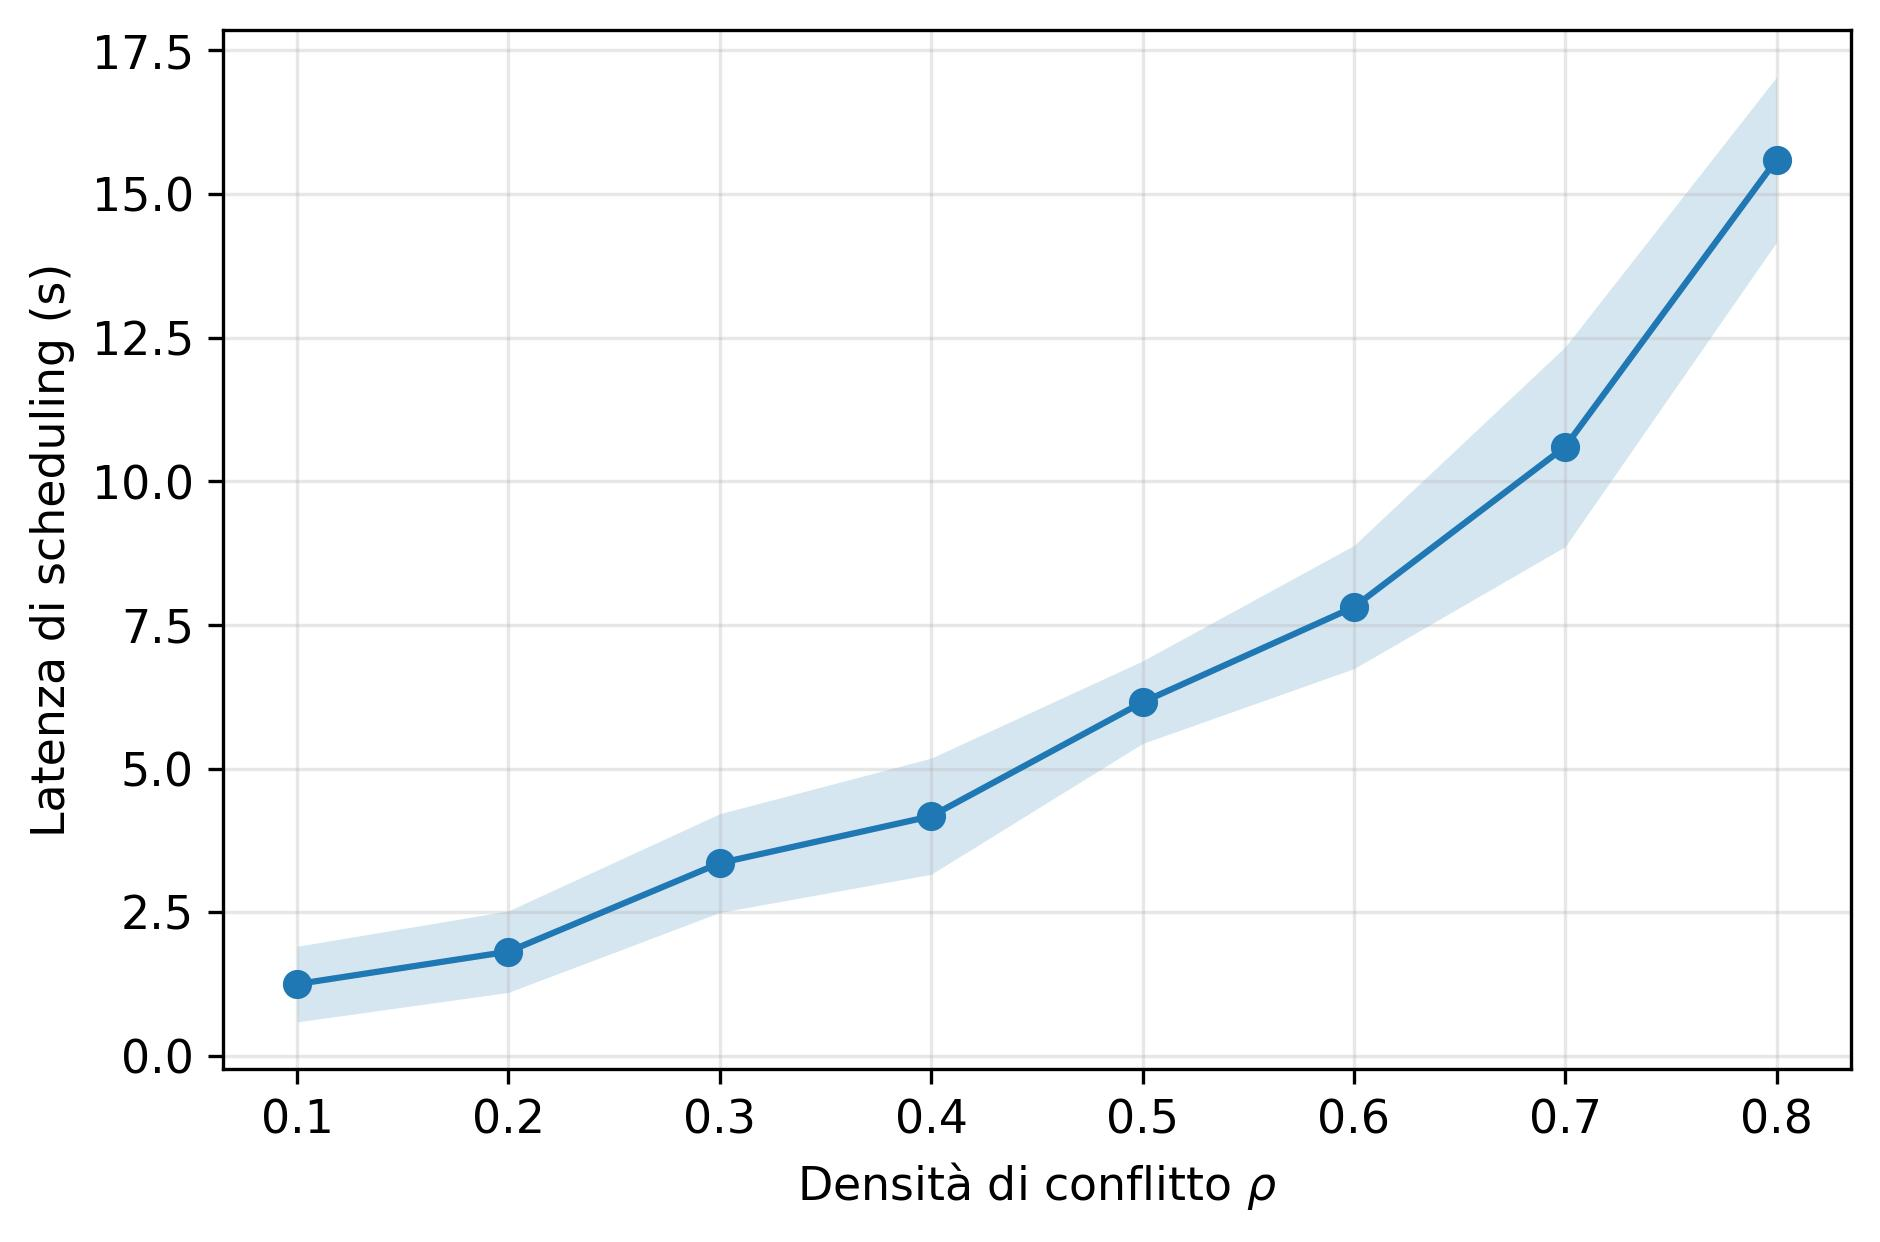
\includegraphics[width=\textwidth]{immagini/val_conflitti/conflicts_latenza.jpg}
        \caption{Latenza media di scheduling.}
        \label{fig:conflitti-latenza}
    \end{subfigure}
    \hfill
    \begin{subfigure}[b]{0.48\textwidth}
        \centering
        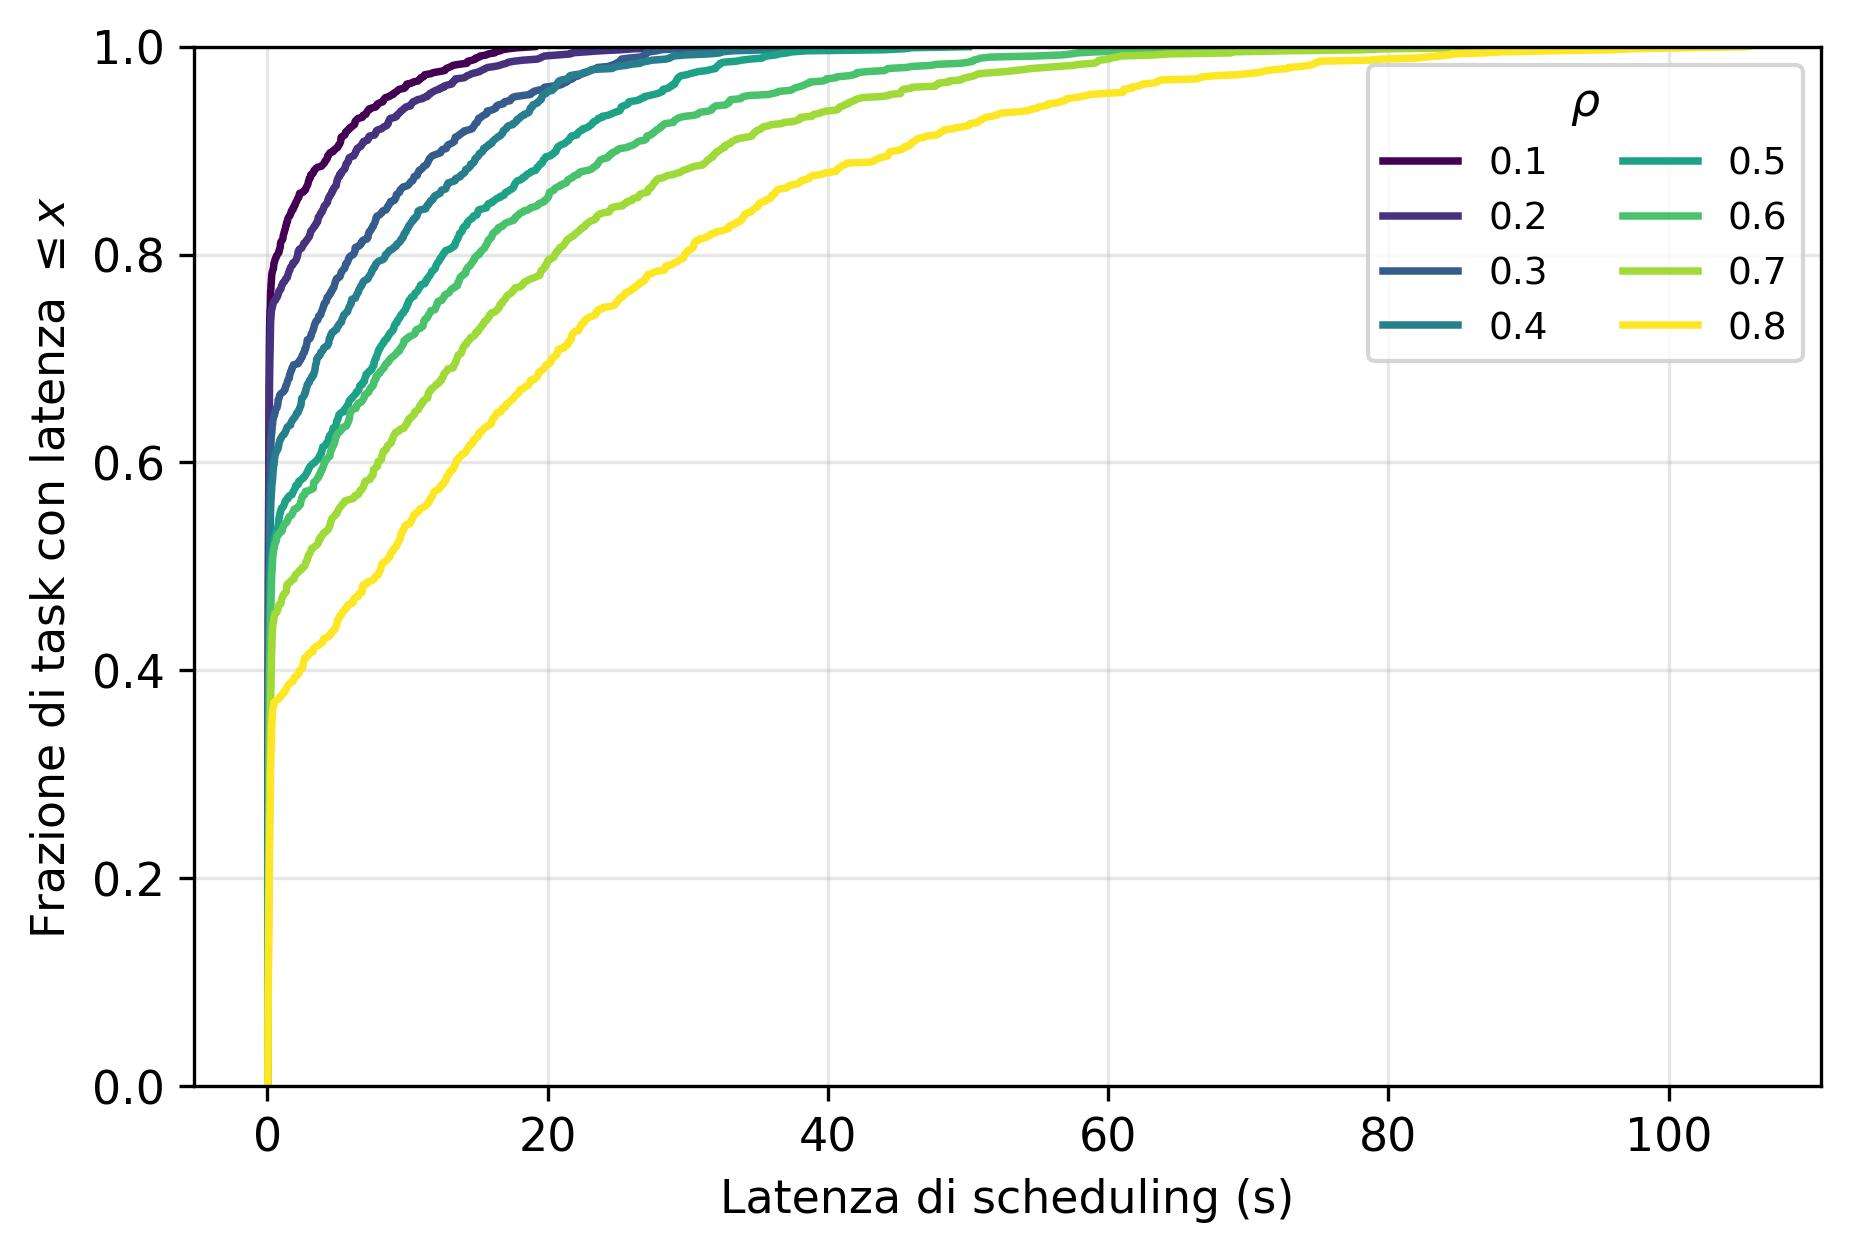
\includegraphics[width=\textwidth]{immagini/val_conflitti/conflicts_cdf.jpg}
        \caption{Distribuzione cumulata della latenza.}
        \label{fig:conflitti-cdf}
    \end{subfigure}
    \caption{Latenza di scheduling al variare della densità di conflitto $\rho$.}
    \label{fig:conflitti-latenza-cdf}
\end{figure}

Il primo effetto da osservare è quello sulla latenza di scheduling, mostrata nella Figura~\ref{fig:conflitti-latenza-cdf} sia come media tra le repliche sia come distribuzione cumulata. La latenza media cresce in modo monotono lungo tutta la griglia, da circa 1.2 secondi a $\rho = 0.1$ fino a 15.6 secondi a $\rho = 0.8$, con una crescita che si fa più ripida alle densità alte. L'andamento è coerente con l'aspettativa formulata nella Sezione~\ref{subsec:perimetro_valutazione} ed è confermato dai test statistici condotti sulle latenze medie delle singole repliche. Il test di Kruskal–Wallis indica che la densità ha un effetto significativo sulla latenza ($H = 37.08$, $p < 10^{-5}$), e la correlazione di Spearman tra densità e latenza conferma che la crescita è monotona e sistematica su tutta la griglia e non frutto di oscillazioni casuali ($r_s = 0.97$, $p < 10^{-24}$). La distribuzione cumulata nella stessa figura mostra la stessa crescita vista dall'intera popolazione dei task. Ogni curva sale rapidamente vicino all'origine, dove si trovano i task schedulati quasi subito, per poi distendersi in una coda che raccoglie i task in attesa di sanificazione. Al crescere di $\rho$ il tratto iniziale si abbassa, perché una quota minore di task passa senza attese, e la coda si allunga verso destra, perché chi viene bloccato attende di più. 

\begin{figure}[htb]
    \centering
    \begin{subfigure}[b]{0.48\textwidth}
        \centering
        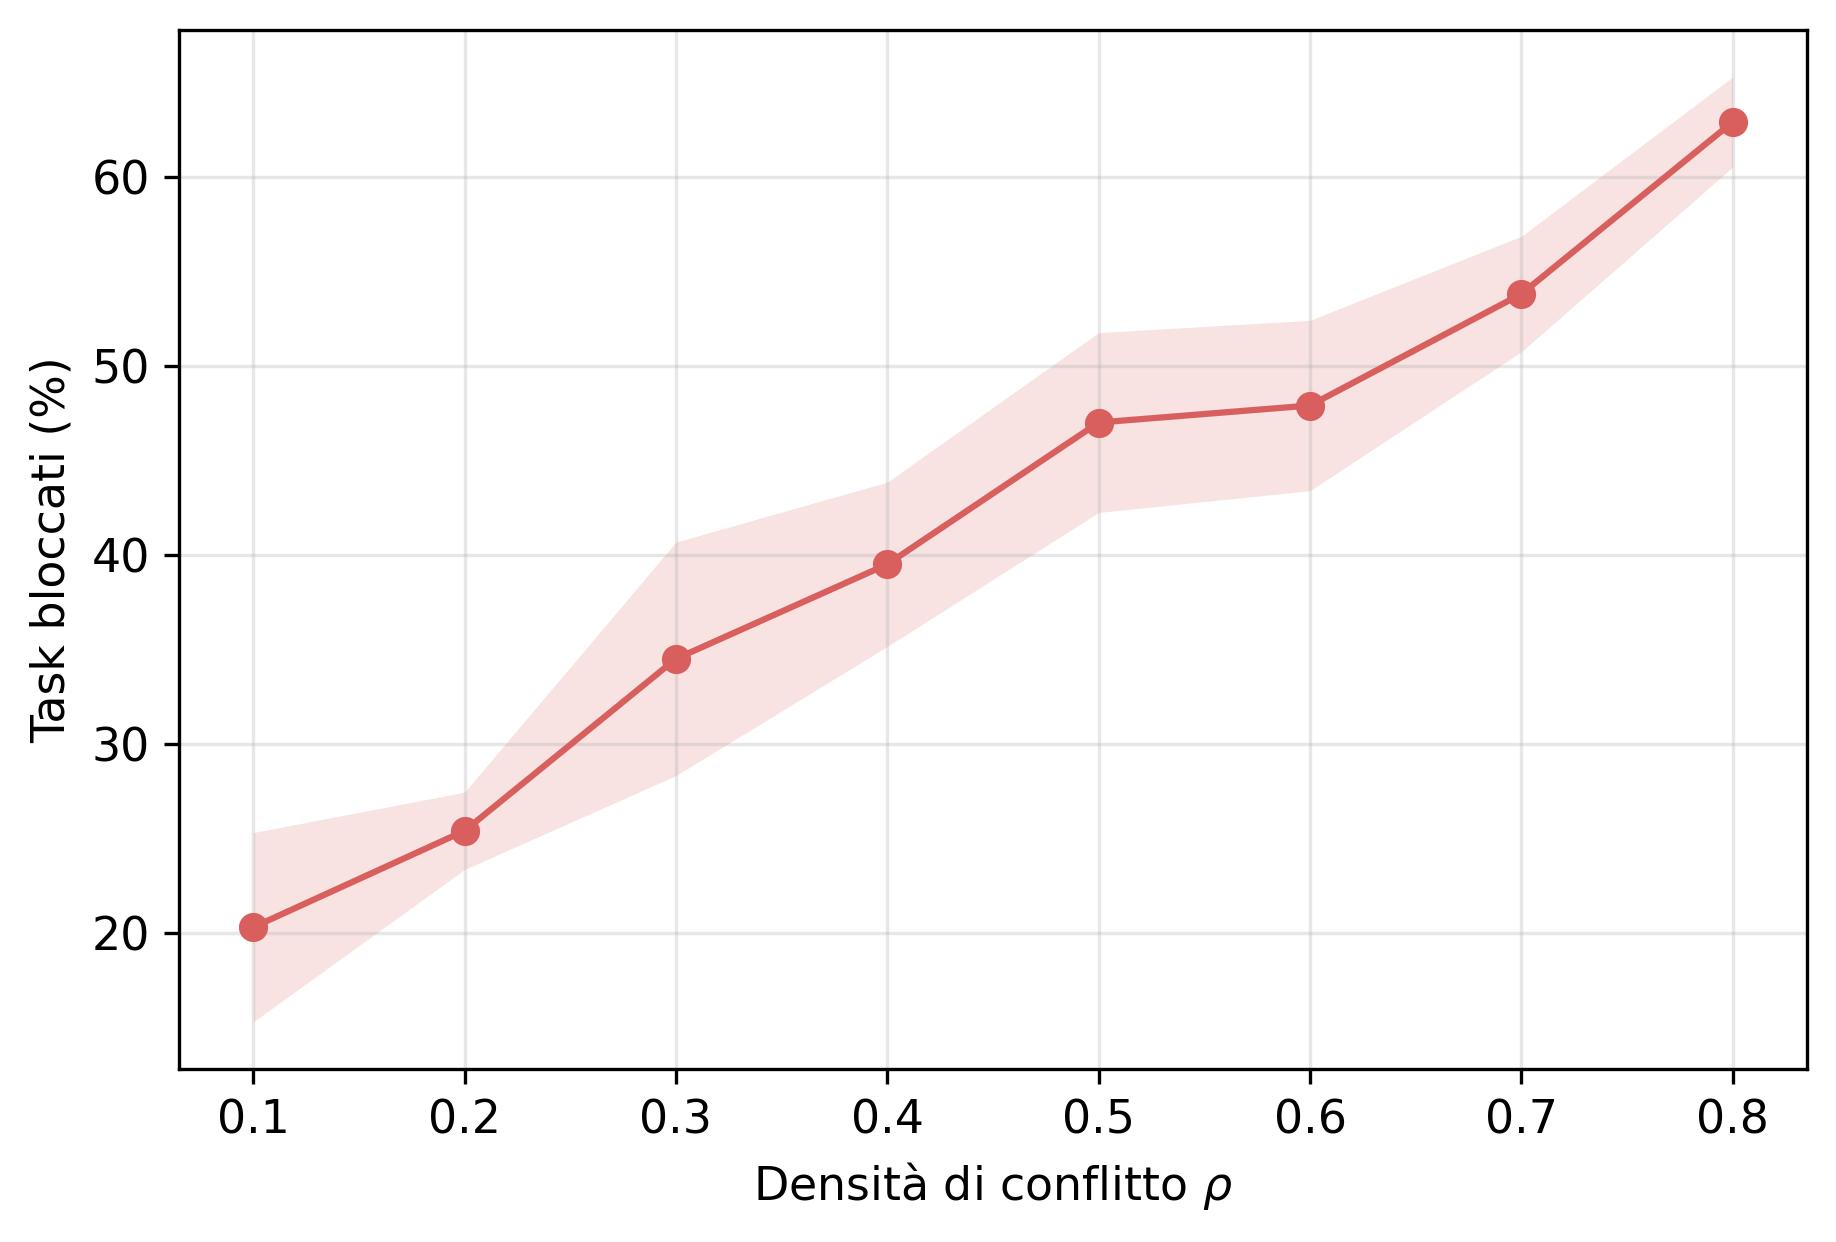
\includegraphics[width=\textwidth]{immagini/val_conflitti/conflicts_bloccati.jpg}
        \caption{Frazione di task bloccati.}
        \label{fig:conflitti-bloccati}
    \end{subfigure}
    \hfill
    \begin{subfigure}[b]{0.48\textwidth}
        \centering
        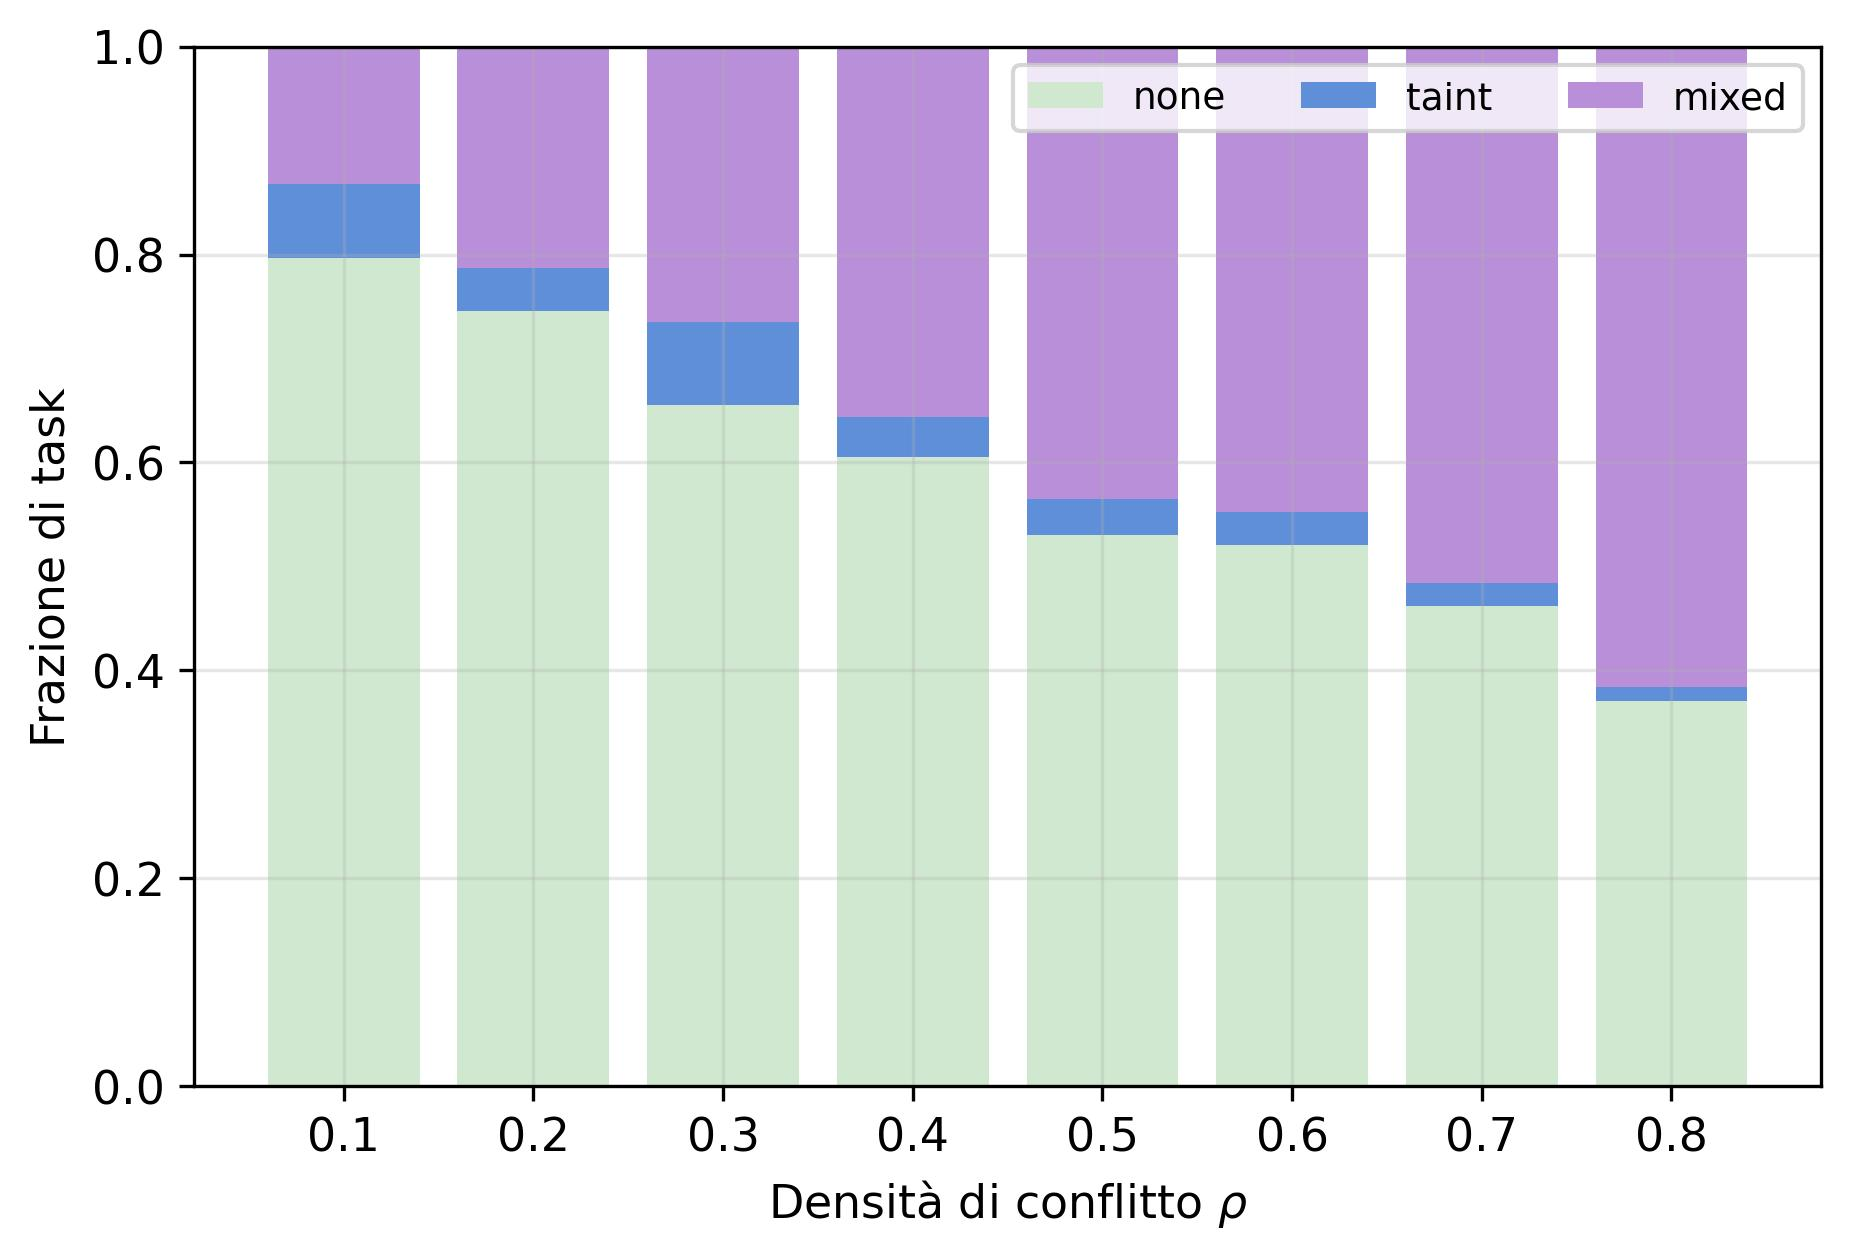
\includegraphics[width=\textwidth]{immagini/val_conflitti/conflicts_cause_blocco.jpg}
        \caption{Ripartizione dei task per causa di blocco.}
        \label{fig:conflitti-cause}
    \end{subfigure}
    \caption{Blocco dei task al variare della densità di conflitto $\rho$.}
    \label{fig:conflitti-bloccati-cause}
\end{figure}

La crescita osservata è riconducibile alla frazione di task bloccati, cioè respinti almeno una volta prima di essere assegnati, che cresce regolarmente dal 20\% a $\rho = 0.1$ fino al 63\% a $\rho = 0.8$, come mostra la Figura~\ref{fig:conflitti-bloccati-cause}. 
È su questa grandezza che la densità di conflitto agisce direttamente, dato che la densità non allunga di per sé l'attesa di un singolo task, ma rende più probabile che un task venga bloccato e debba quindi attendere un nuovo tentativo di assegnazione.

Di fianco, la ripartizione per causa distingue tutti i task della run in base a ciò che hanno incontrato prima di essere assegnati. La quota segnata come \emph{none} raccoglie i task assegnati al primo tentativo, senza alcun blocco; quella segnata come \emph{taint} i task esclusi perché il nodo era in sanificazione, e quella marcata come \emph{mixed} i task che nel corso della loro attesa hanno incontrato sia una traccia in conflitto sia la procedura di sanificazione. Gli ultimi due casi sono in realtà due facce dello stesso fenomeno, perché la traccia contestuale che blocca un task viene rimossa proprio dalla sanificazione del nodo, e durante quella finestra il nodo resta escluso per via del \emph{taint}. Per questo un task che attende la pulizia di un nodo attraversa quasi sempre entrambe le cause e ricade in \emph{mixed}, mentre i blocchi dovuti al solo \emph{taint} restano una quota minore. Ciò che conta, ai fini dell'esperimento, è che i task bloccati solamente dal \emph{taint} non crescono con $\rho$, ma restano una quota contenuta che tende anzi a ridursi, dato che l'intervallo $\tau$ è fisso. Quindi, a crescere è soltanto il blocco dovuto alle tracce in conflitto, confermando che l'aumento di latenza dipende solamente dai conflitti e non dalla sanificazione, che in questo caso è costante.

\begin{figure}[htb]
    \centering
    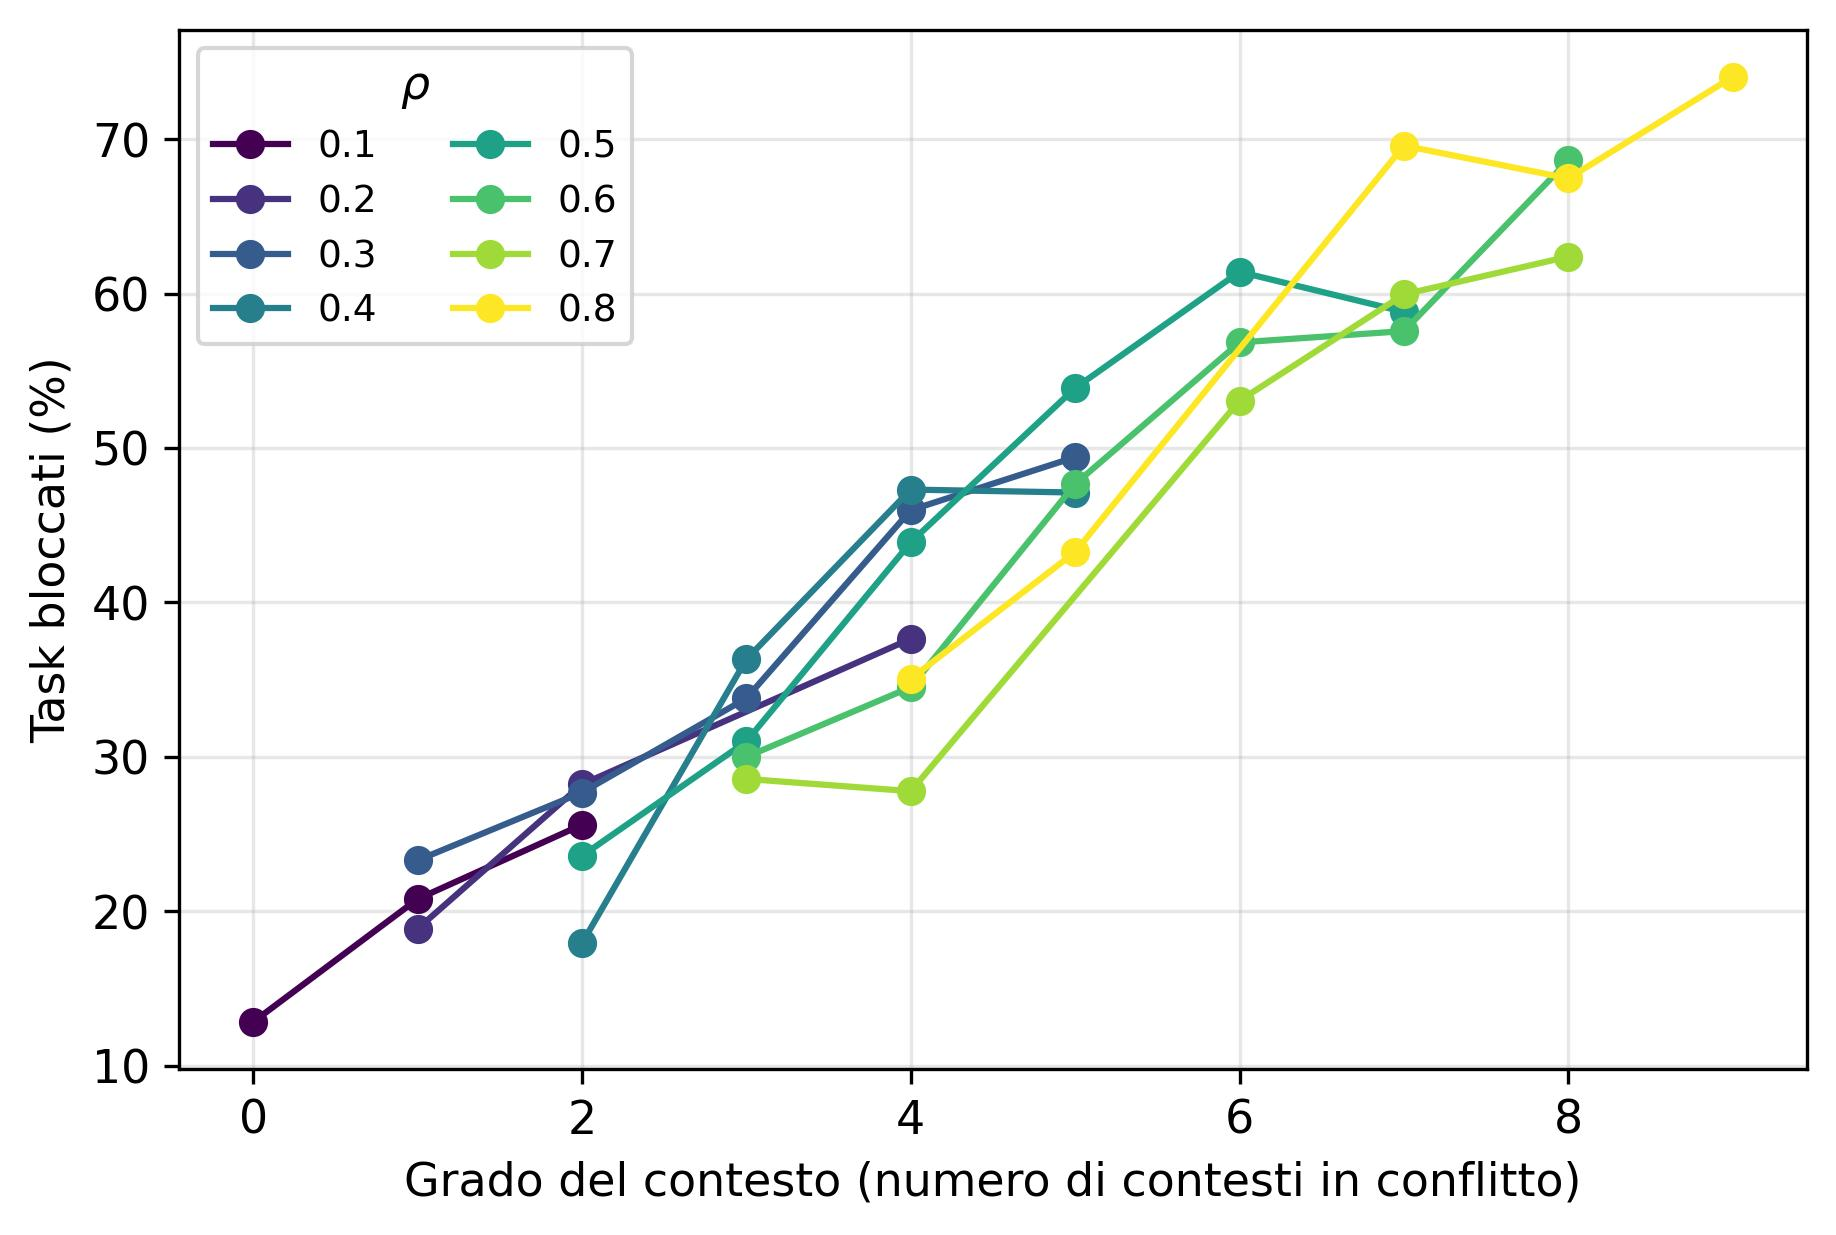
\includegraphics[width=0.48\textwidth]{immagini/val_conflitti/conflicts_grado.jpg}
    \caption{Frazione di task bloccati in funzione del grado del contesto.}
    \label{fig:conflitti-grado}
\end{figure}

Resta da capire perché sia la densità a far salire il numero di blocchi, e la Figura~\ref{fig:conflitti-grado} lo chiarisce riportando la frazione di task bloccati in funzione del grado del contesto richiesto. Le curve delle diverse densità tendono a sovrapporsi lungo un'unica tendenza comune, dato che a parità di grado un task viene bloccato con la stessa frequenza qualunque sia la densità dello scenario. Il blocco non dipende quindi dalla densità in sé, ma dal grado del contesto del task, e la densità agisce sulla latenza proprio perché, aumentando, fa salire il grado medio dei contesti.

\begin{figure}[htb]
    \centering
    \begin{subfigure}[b]{0.48\textwidth}
        \centering
        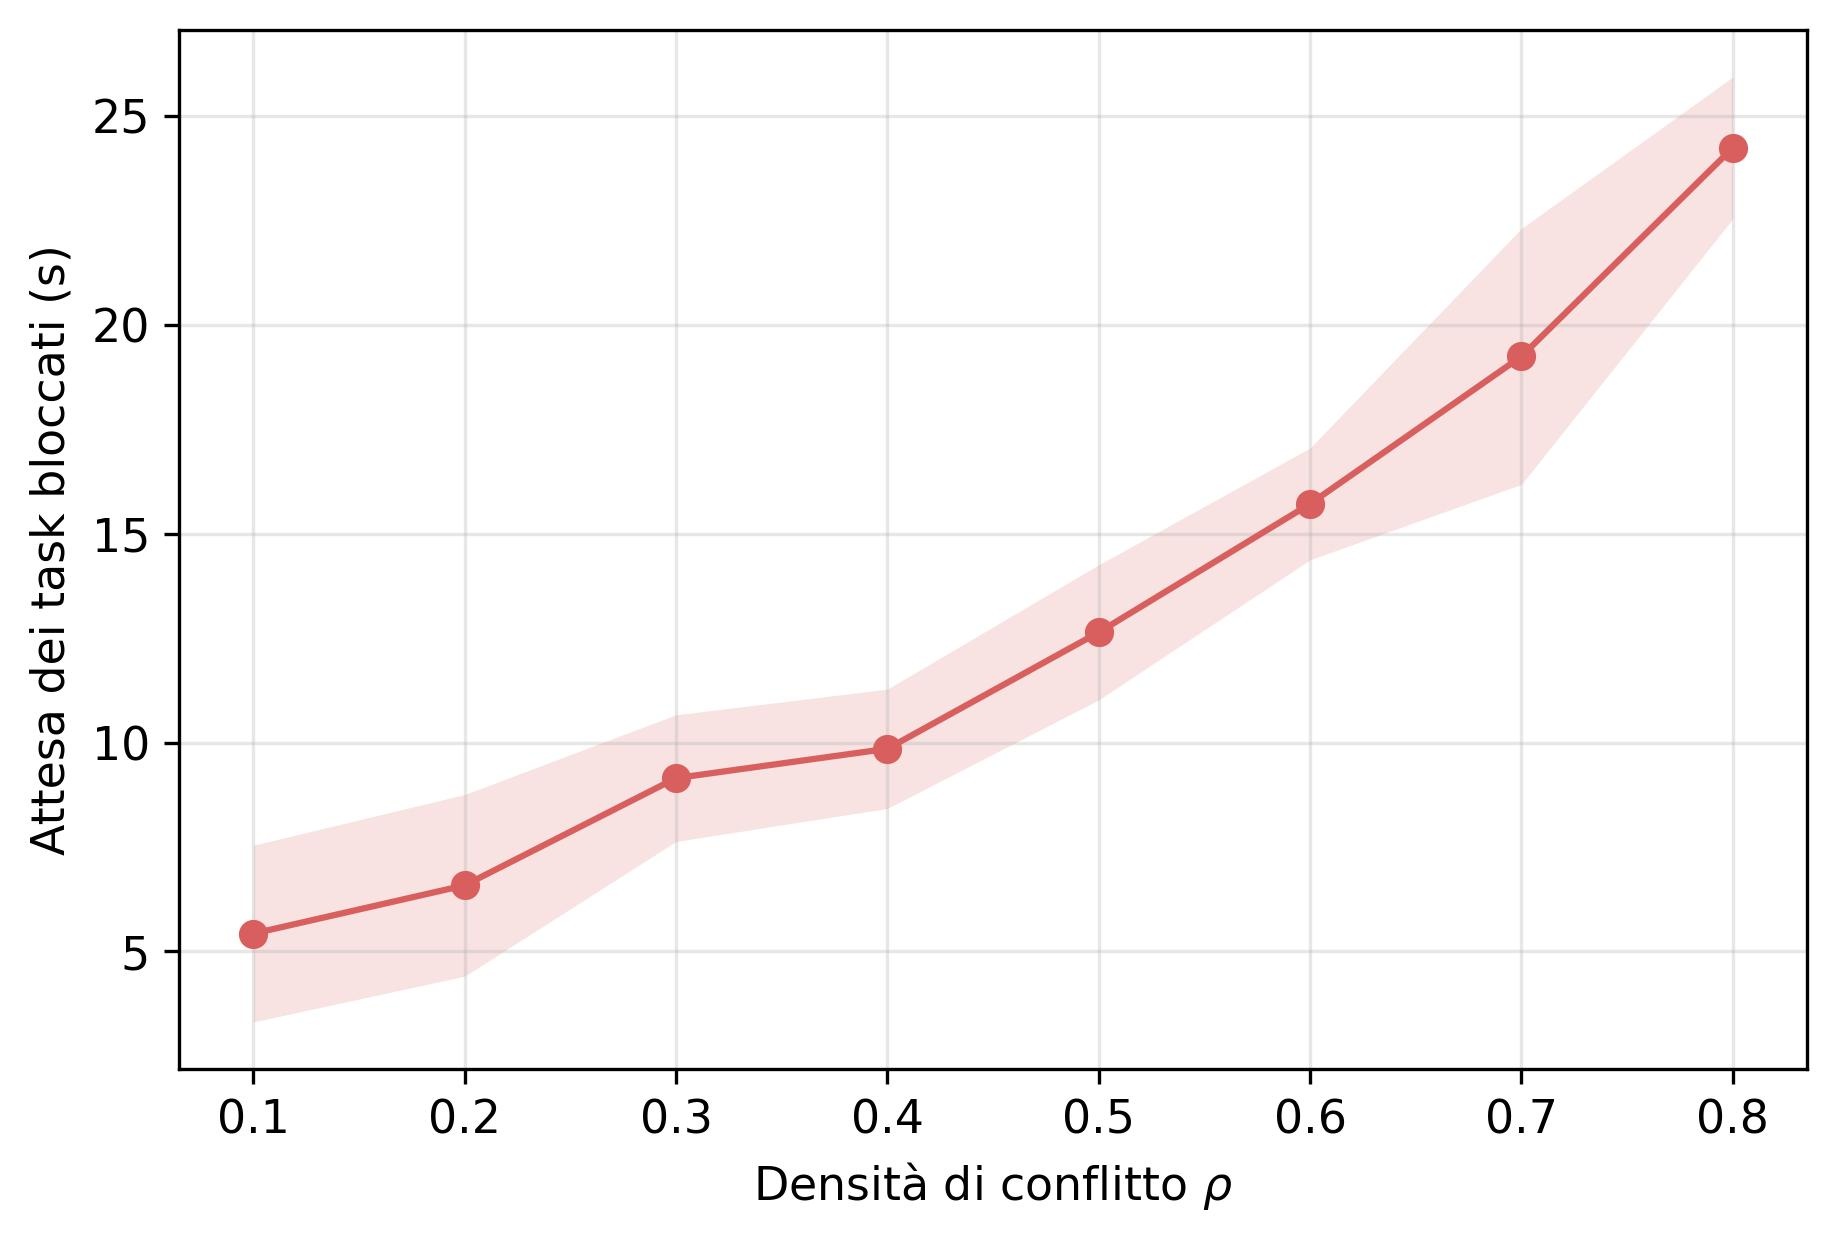
\includegraphics[width=\textwidth]{immagini/val_conflitti/conflicts_attesa.jpg}
        \caption{Attesa media dei task bloccati.}
        \label{fig:conflitti-attesa}
    \end{subfigure}
    \hfill
    \begin{subfigure}[b]{0.48\textwidth}
        \centering
        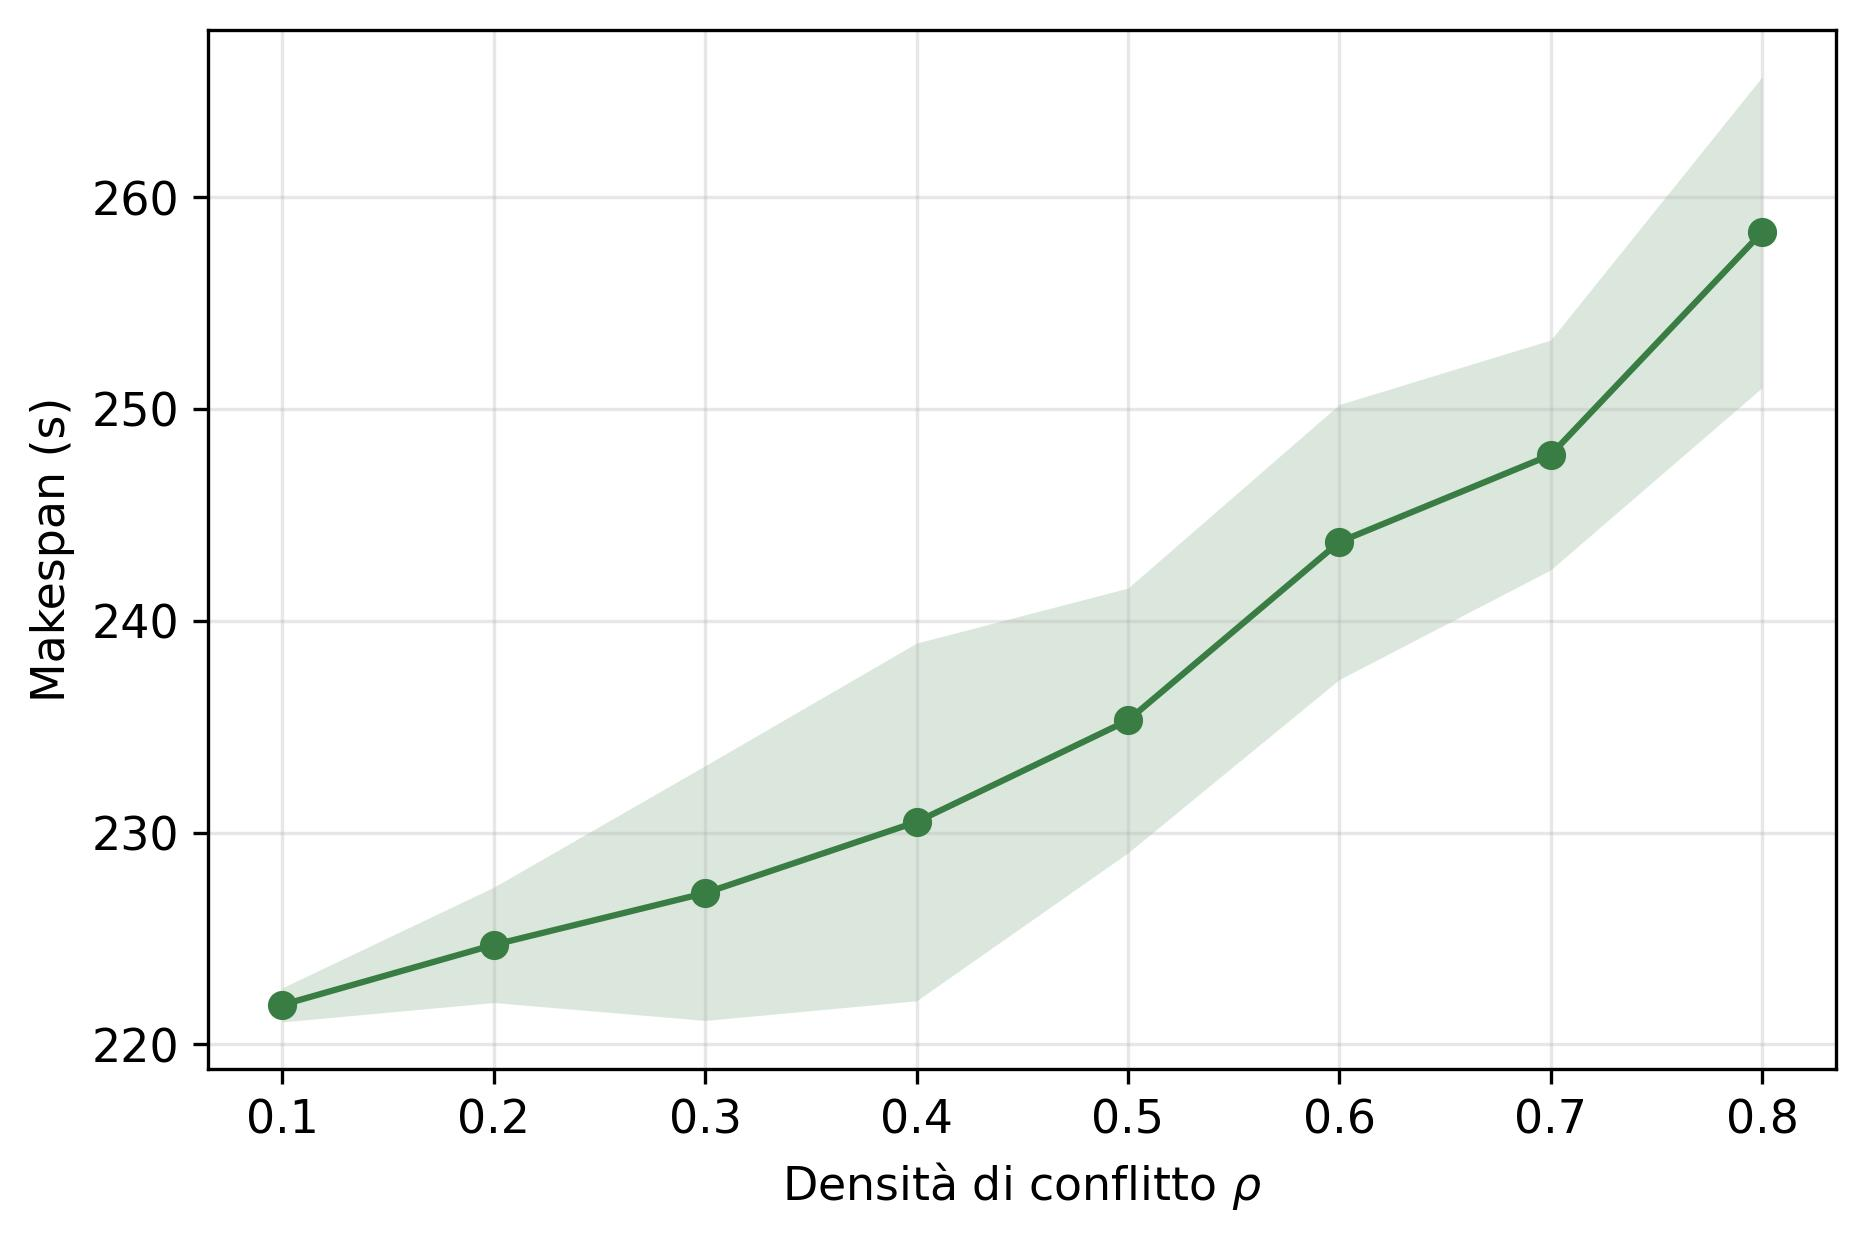
\includegraphics[width=\textwidth]{immagini/val_conflitti/conflicts_makespan.jpg}
        \caption{Makespan del batch.}
        \label{fig:conflitti-makespan}
    \end{subfigure}
    \caption{Costo globale dei conflitti al variare della densità $\rho$.}
    \label{fig:conflitti-attesa-makespan}
\end{figure}

Oltre alla probabilità di blocco, i conflitti incidono anche sul tempo, che la Figura~\ref{fig:conflitti-attesa-makespan} mostra da due prospettive diverse. L'attesa media dei task bloccati, dal primo rifiuto fino al binding, cresce da circa 5 secondi a $\rho = 0.1$ fino a oltre 24 secondi a $\rho = 0.8$: a densità più alta un task bloccato trova contaminati più nodi e deve attendere che un numero maggiore di essi venga ripulito prima di trovarne uno compatibile. Il makespan, ovvero il tempo per completare l'intero batch di 200 task, cresce anch'esso ma molto più lentamente, da circa 222 a 258 secondi, perché include per costruzione i 200 secondi di sottomissione e perché le attese dei task bloccati si sovrappongono nel tempo invece di sommarsi, dato che molti task attendono lo stesso ciclo di sanificazione. Le due viste restano entrambe utili, perché la prima misura il costo percepito da chi sottomette e la seconda quello complessivo sostenuto dal cluster.

Nel complesso, l'esperimento conferma che la latenza di scheduling cresce in modo monotono e significativo con la densità di conflitto, e individua nel grado dei singoli contesti, più che nella densità complessiva, la grandezza che governa il fenomeno.

% ------------------------------------------------------------ %

\section{Impatto dell'Intervallo di Sanificazione}
\label{sec:impatto_intervallo}

Il secondo esperimento fa variare l'intervallo di sanificazione $\tau$ tra 1 e 50 secondi mantenendo fissa la densità di conflitto a $\rho = 0.5$, un valore intermedio che garantisce una quota di task bloccati sufficiente a rendere osservabile l'effetto della sanificazione senza saturare il sistema. A differenza della densità di conflitto, che agisce sulla probabilità di blocco, l'intervallo agisce sul tempo che un task bloccato attende prima di potersi schedulare, e il suo effetto non è monotono.

\begin{figure}[htb]
    \centering
    \begin{subfigure}[b]{0.48\textwidth}
        \centering
        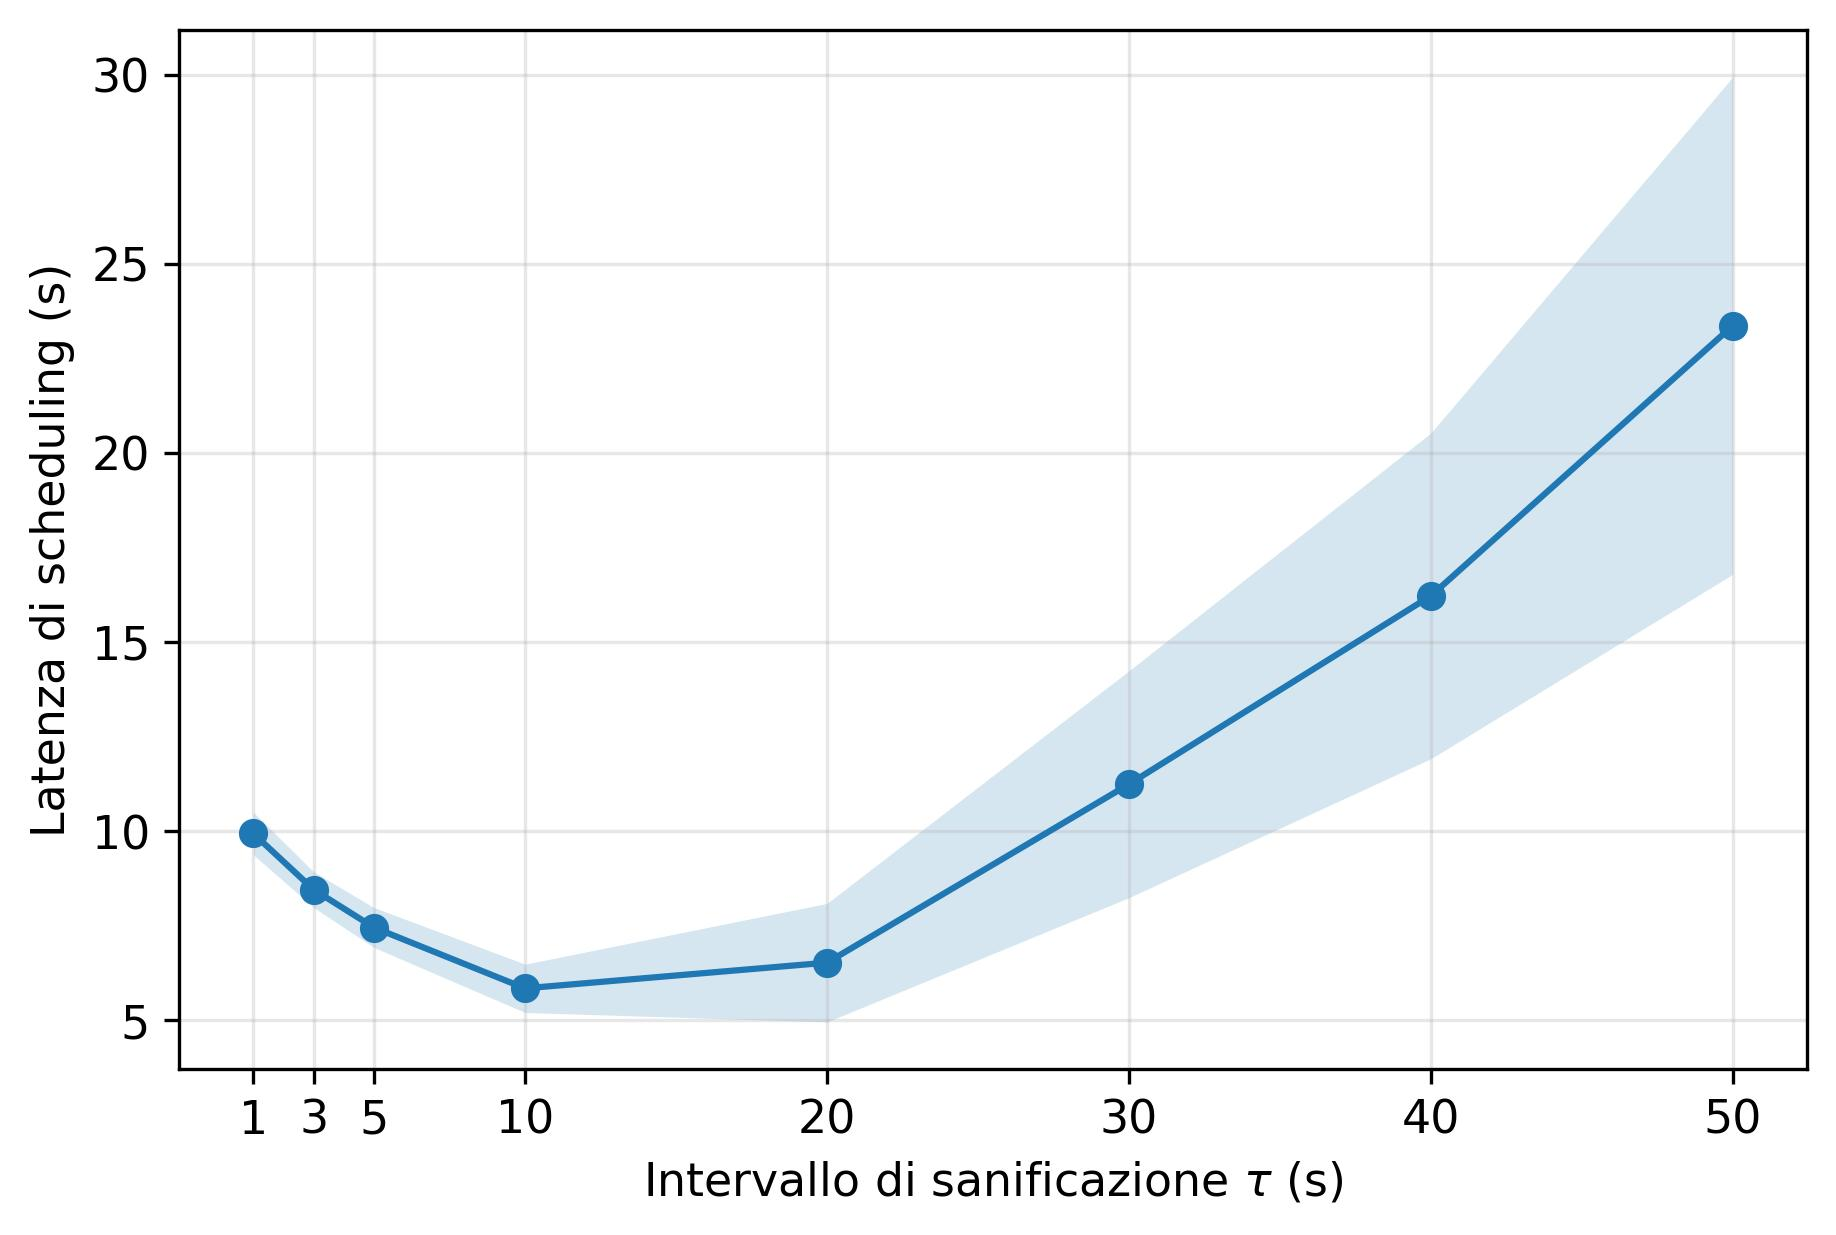
\includegraphics[width=\textwidth]{immagini/val_sanificazione/sanitize_latenza.jpg}
        \caption{Latenza media di scheduling.}
        \label{fig:sanificazione-latenza}
    \end{subfigure}
    \hfill
    \begin{subfigure}[b]{0.48\textwidth}
        \centering
        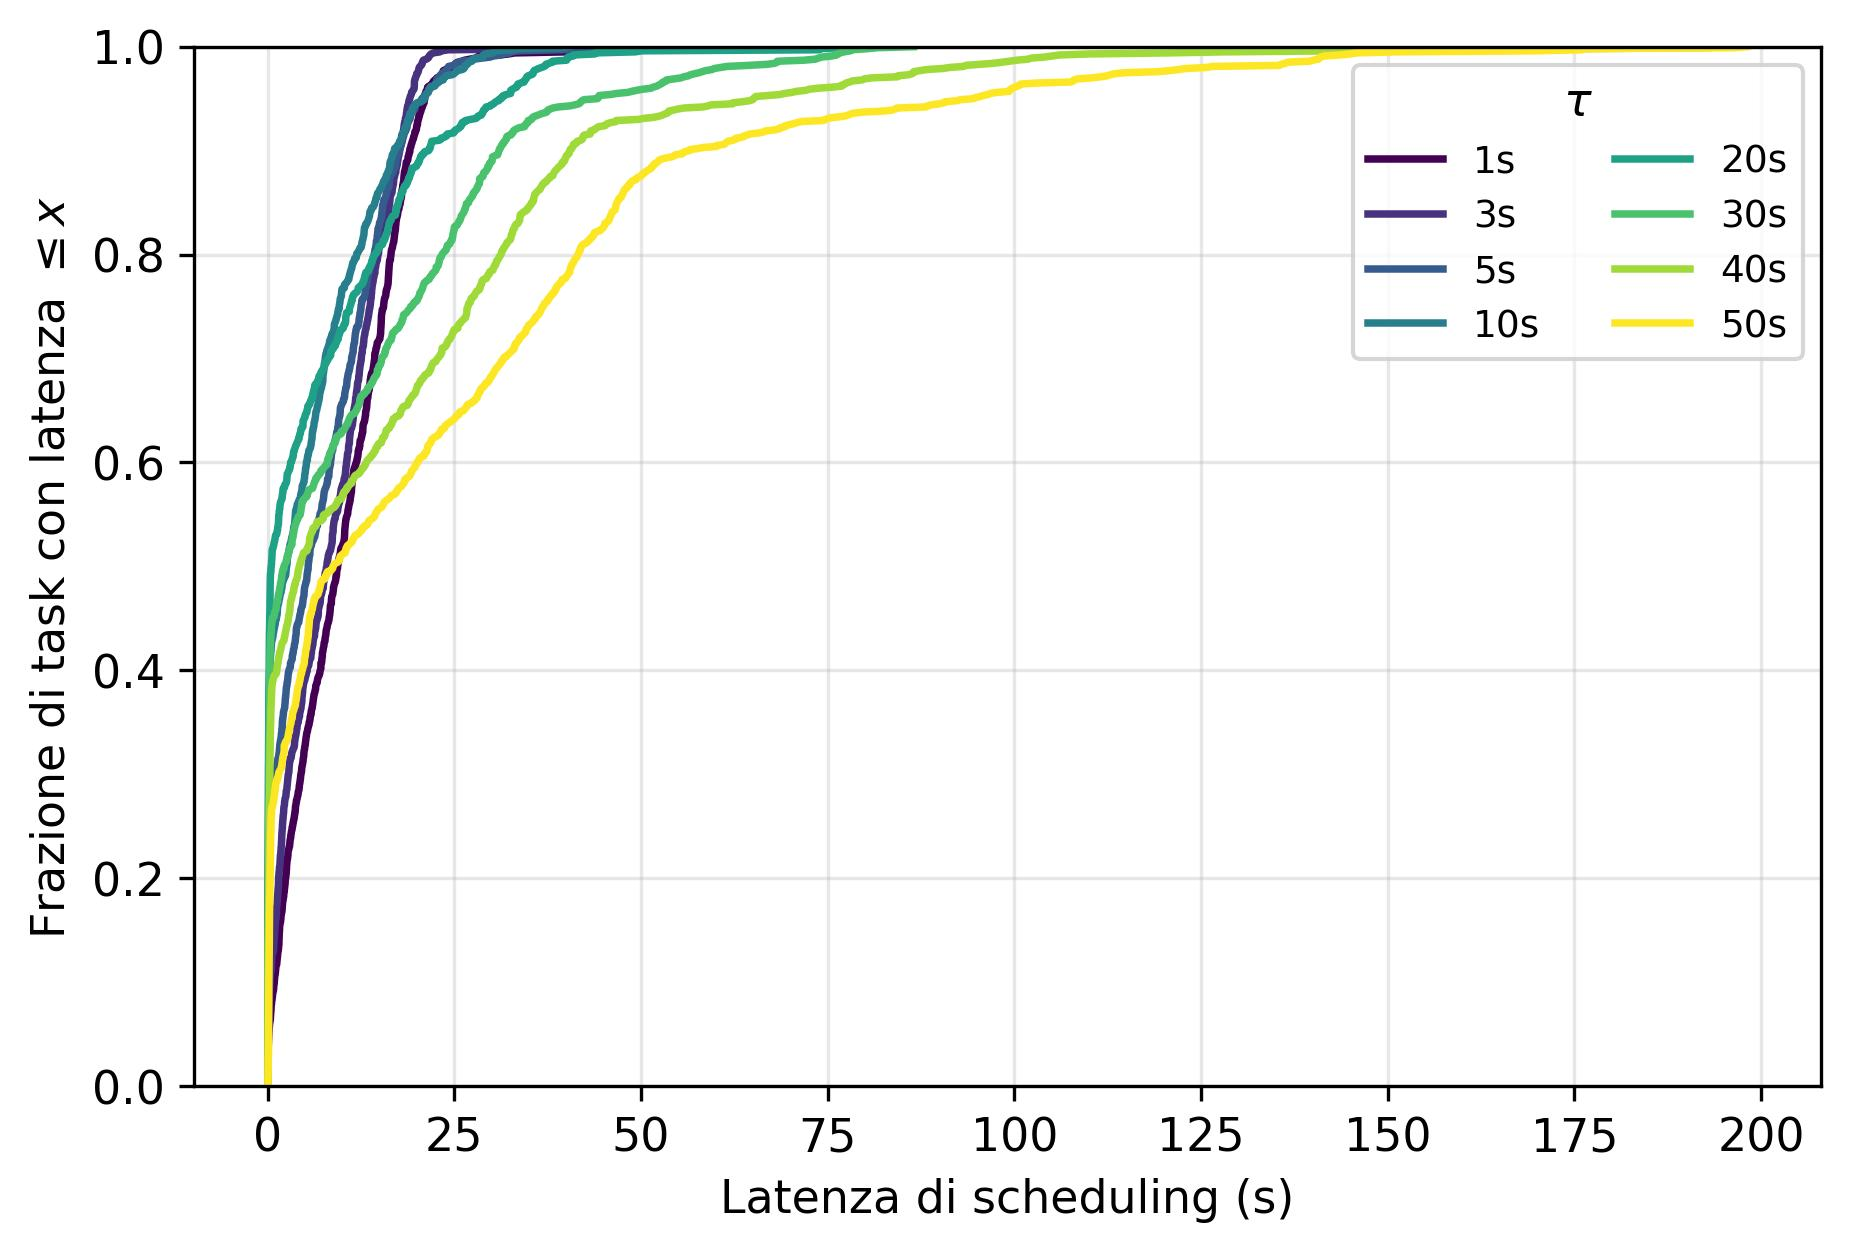
\includegraphics[width=\textwidth]{immagini/val_sanificazione/sanitize_cdf.jpg}
        \caption{Distribuzione cumulata della latenza.}
        \label{fig:sanificazione-cdf}
    \end{subfigure}
    \caption{Latenza di scheduling al variare dell'intervallo di sanificazione $\tau$.}
    \label{fig:sanificazione-latenza-cdf}
\end{figure}

La latenza di scheduling, mostrata nella Figura~\ref{fig:sanificazione-latenza-cdf}, conferma l'andamento a U anticipato nella Sezione~\ref{subsec:perimetro_valutazione}. Partendo da circa 10 secondi a $\tau = 1$, la latenza media scende fino a un minimo di 5.8 secondi a $\tau = 10$, per poi risalire e raggiungere oltre 23 secondi a $\tau = 50$. I due bracci della curva hanno origini diverse, discusse più avanti, ma la loro esistenza suggerisce che né sanificare molto spesso né sanificare molto di rado sia la scelta migliore. Un altro aspetto che la curva rende evidente è l'allargarsi della varianza verso destra, perché agli intervalli più lunghi una run contiene pochi cicli di sanificazione e la latenza dipende sempre più da quando esattamente questi cicli cadono rispetto ai task in esecuzione, rendendo la misura meno stabile. Il test di Kruskal–Wallis conferma che l'intervallo ha un effetto significativo sulla latenza ($H = 31.87$, $p < 10^{-4}$), mentre la natura del minimo emerge dai confronti a coppie tra valori adiacenti di $\tau$, condotti con il test di Mann–Whitney a due code sulle latenze medie delle singole repliche. La latenza a $\tau = 10$ risulta significativamente inferiore a quella a $\tau = 5$ ($U = 0$, $p < 10^{-2}$) ma non è distinguibile da quella a $\tau = 20$ ($U = 9$, $p = 0.90$), che a sua volta è inferiore a quella a $\tau = 30$ ($U = 1$, $p = 0.03$). L'ottimo non è quindi un singolo valore, ma una regione compresa tra $\tau = 10$ e $\tau = 20$, ai cui estremi le prestazioni non risultano statisticamente distinguibili. La distribuzione cumulata mostra lo stesso andamento dal punto di vista dei singoli task. Agli intervalli brevi il tratto iniziale è basso, perché pochi task trovano un nodo disponibile al primo tentativo, ma la coda è corta, perché i nodi tornano disponibili in fretta. Tra $\tau = 10$ e $\tau = 20$ il tratto iniziale raggiunge la sua altezza massima, mentre agli intervalli lunghi si abbassa di nuovo e la coda si allunga verso destra, fino a superare gli 80 secondi a $\tau = 50$.

\begin{figure}[htb]
    \centering
    \begin{subfigure}[b]{0.48\textwidth}
        \centering
        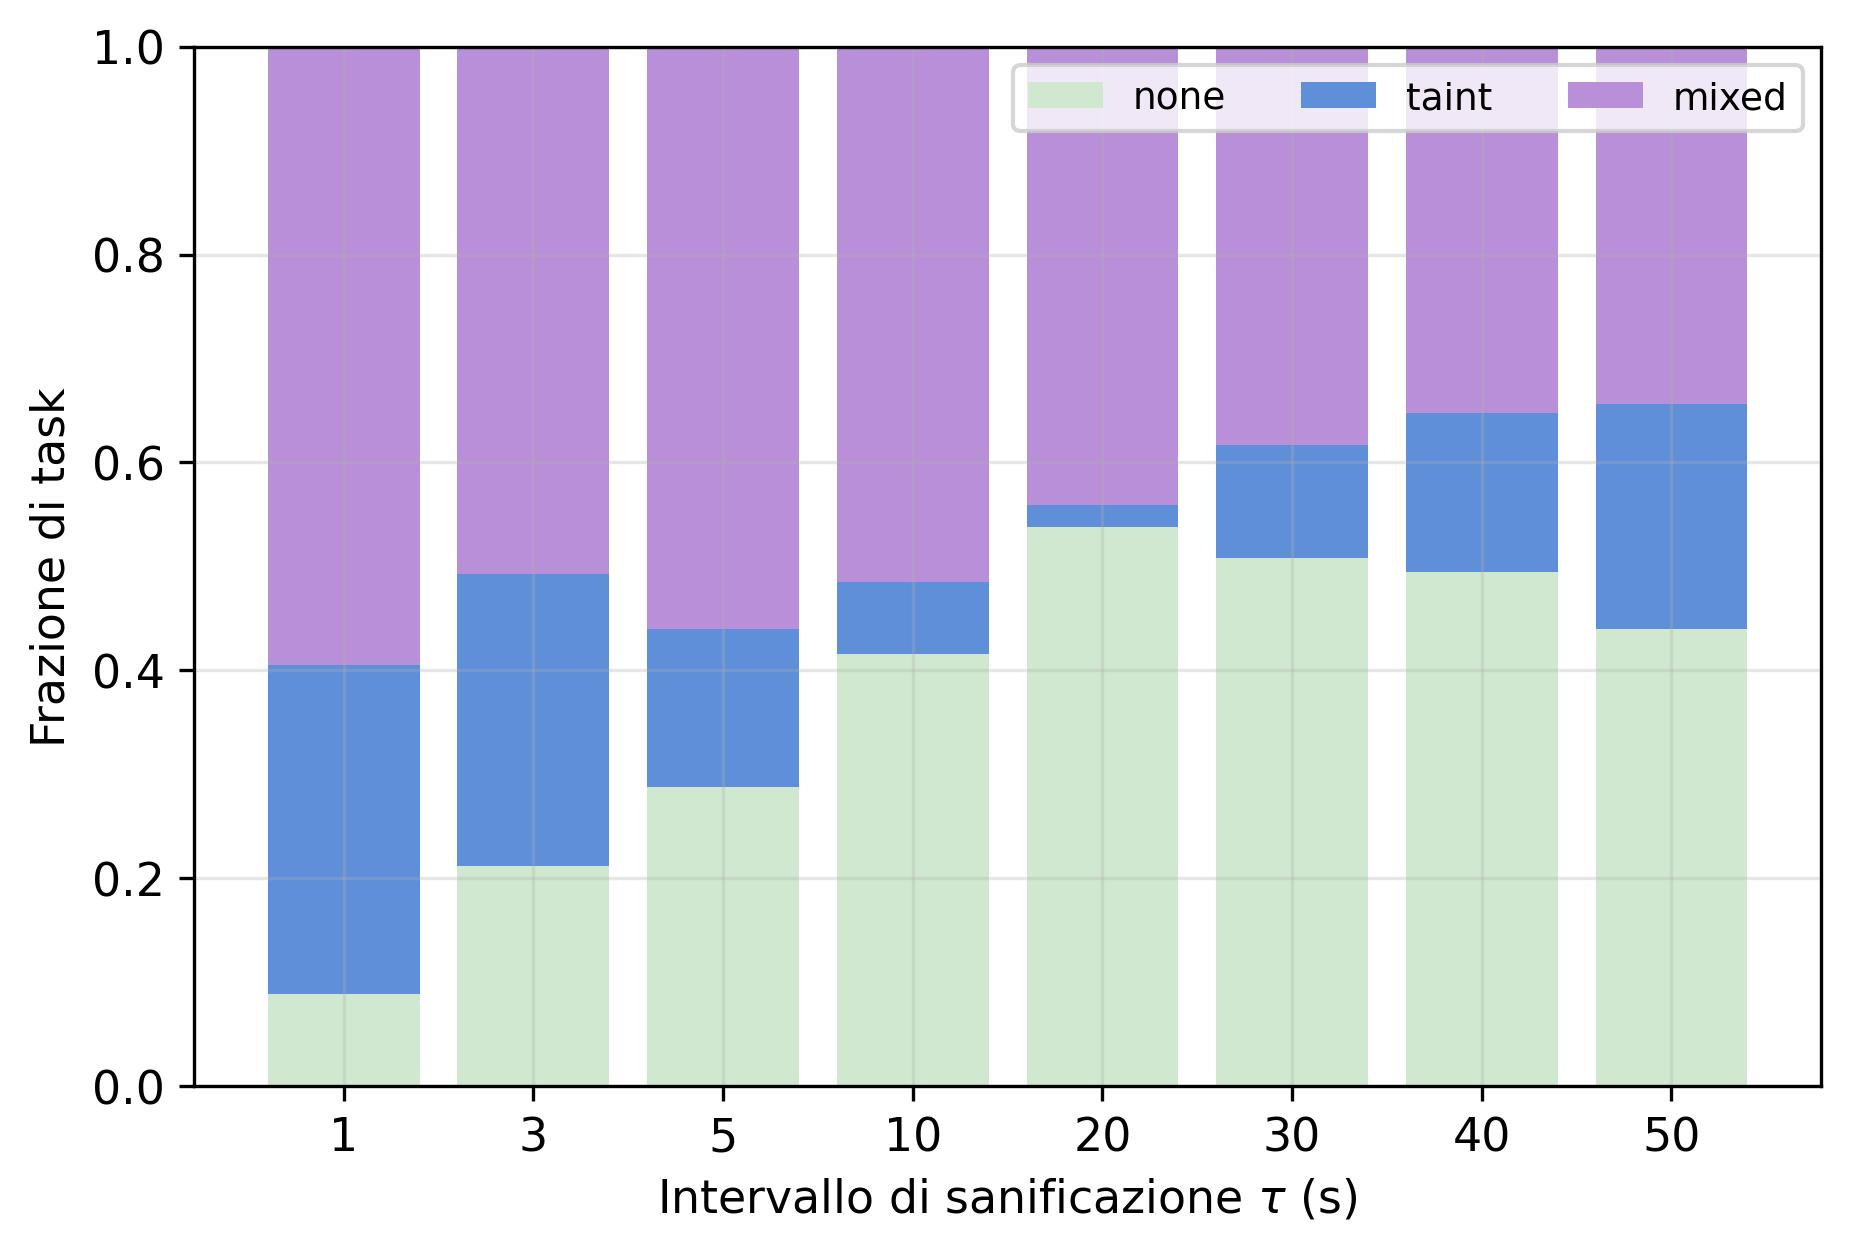
\includegraphics[width=\textwidth]{immagini/val_sanificazione/sanitize_cause_blocco.jpg}
        \caption{Ripartizione dei task per causa di blocco.}
        \label{fig:sanificazione-cause}
    \end{subfigure}
    \hfill
    \begin{subfigure}[b]{0.48\textwidth}
        \centering
        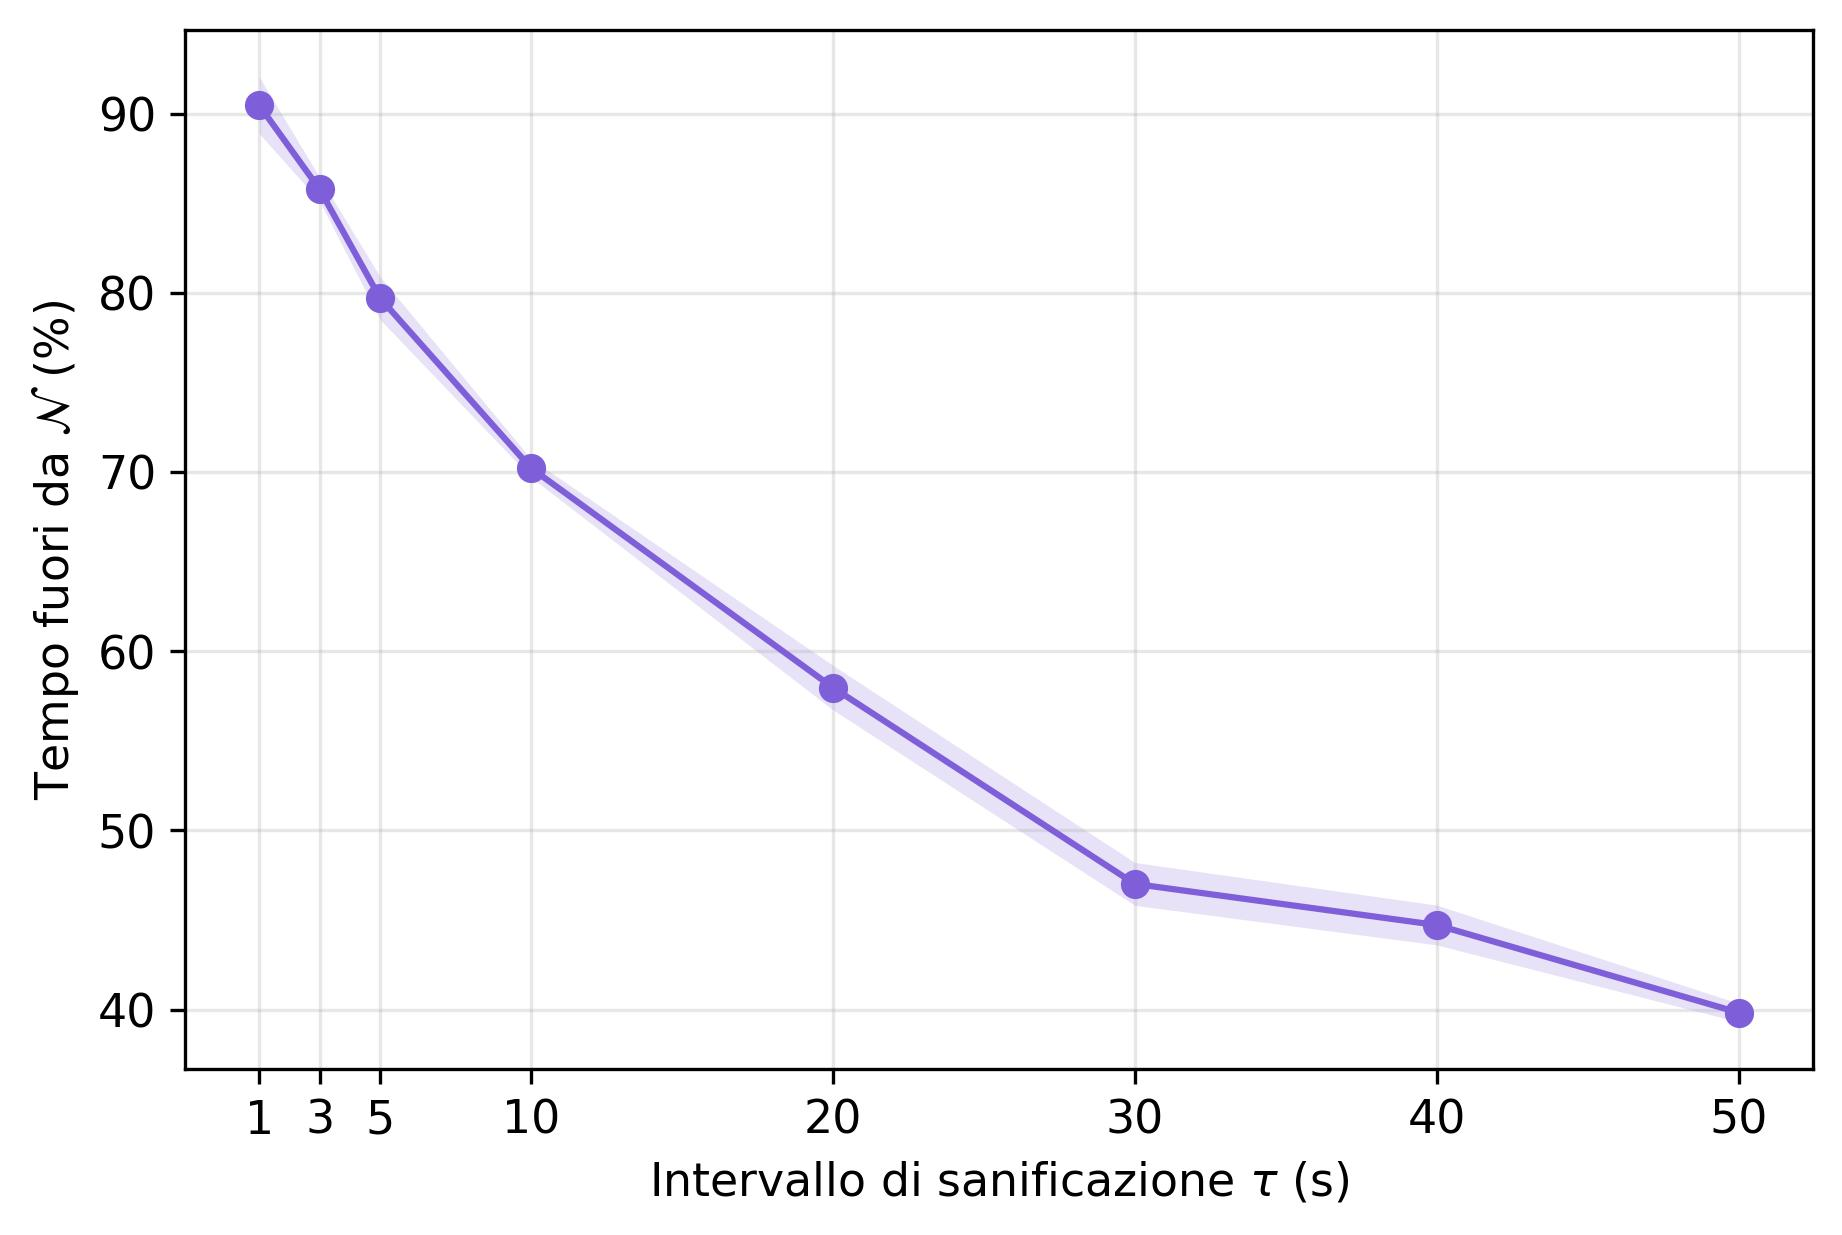
\includegraphics[width=\textwidth]{immagini/val_sanificazione/sanitize_disponibilita.jpg}
        \caption{Indisponibilità media dei nodi.}
        \label{fig:sanificazione-disponibilita}
    \end{subfigure}
    \caption{Cause del blocco dei task e indisponibilità dei nodi al variare dell'intervallo $\tau$.}
    \label{fig:sanificazione-cause-disponibilita}
\end{figure}

La ragione dei due bracci emerge dalla Figura~\ref{fig:sanificazione-cause-disponibilita}, che spiega il fenomeno dai due lati, quello dei task e quello dei nodi. A sinistra, la ripartizione per causa di blocco mostra che agli intervalli più brevi è elevata la quota di task respinti perché il nodo è in sanificazione, segnata come \emph{taint}. Con un intervallo di pochi secondi i nodi vengono messi in sanificazione di continuo, e un task ha alta probabilità di trovarli indisponibili non perché contaminati, ma perché in pulizia. Al crescere di $\tau$ questa componente si riduce fino a quasi annullarsi intorno a $\tau = 20$, dove il blocco è dovuto quasi solo alle tracce contestuali non ancora rimosse, per poi risalire agli intervalli più lunghi. 

Lo stesso fenomeno, visto dal lato dei nodi, è riassunto dall'indisponibilità media, che misura la frazione di tempo in cui un nodo si trova fuori da $\mathcal{N}$ perché in sanificazione. Essa decresce in modo monotono, da oltre il 90\% a $\tau = 1$ fino a circa il 40\% a $\tau = 50$: più spesso si sanifica, più a lungo i nodi restano indisponibili; è proprio questa indisponibilità a spiegare il braccio sinistro della U, mentre agli intervalli lunghi il braccio destro nasce dall'effetto opposto, con le tracce che permangono troppo a lungo e bloccano un numero crescente di task. I due bracci sono quindi le due facce del compromesso tra disponibilità dei nodi e reattività dello scheduling anticipato all'inizio del capitolo.

\begin{figure}[htb]
    \centering
    \begin{subfigure}[b]{0.48\textwidth}
        \centering
        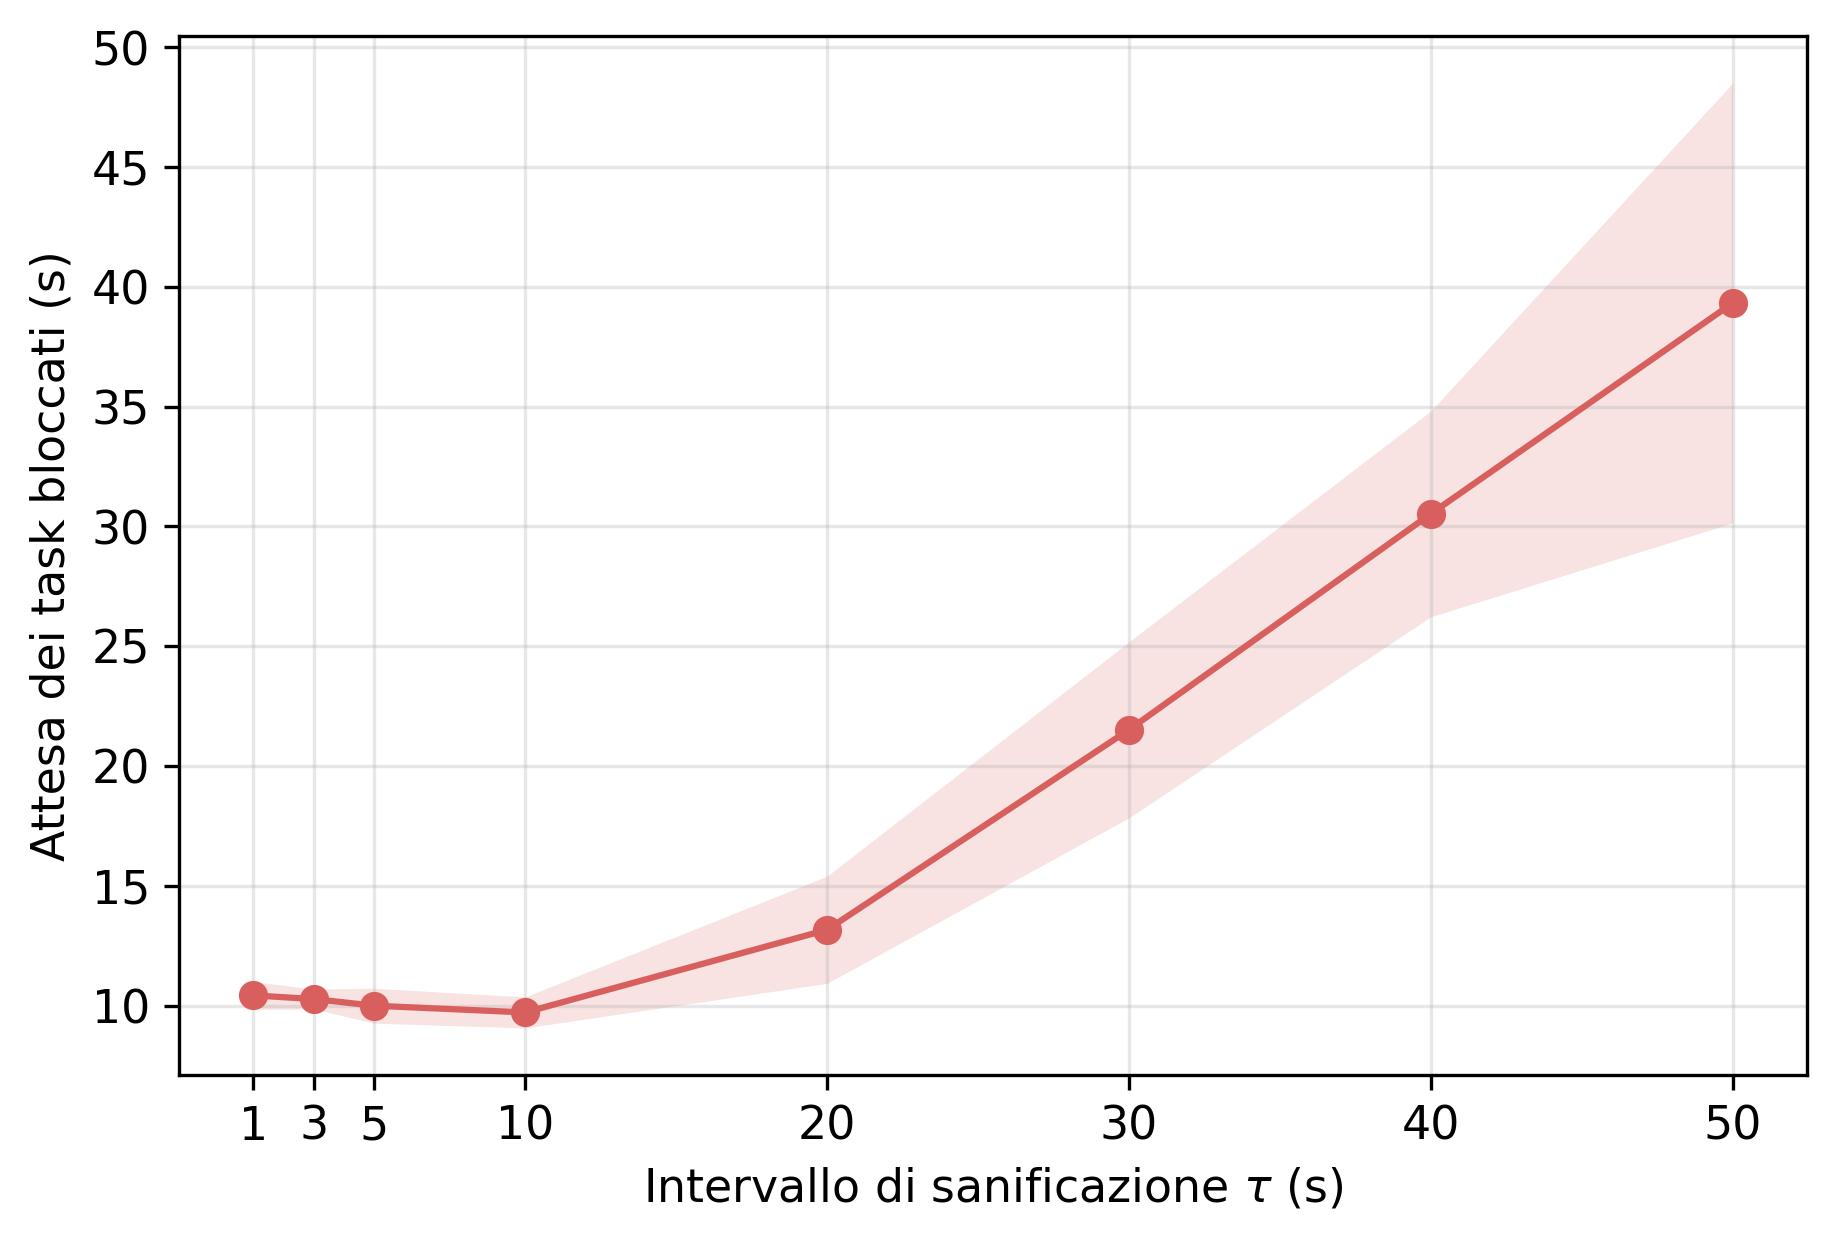
\includegraphics[width=\textwidth]{immagini/val_sanificazione/sanitize_attesa.jpg}
        \caption{Attesa media dei task bloccati.}
        \label{fig:sanificazione-attesa}
    \end{subfigure}
    \hfill
    \begin{subfigure}[b]{0.48\textwidth}
        \centering
        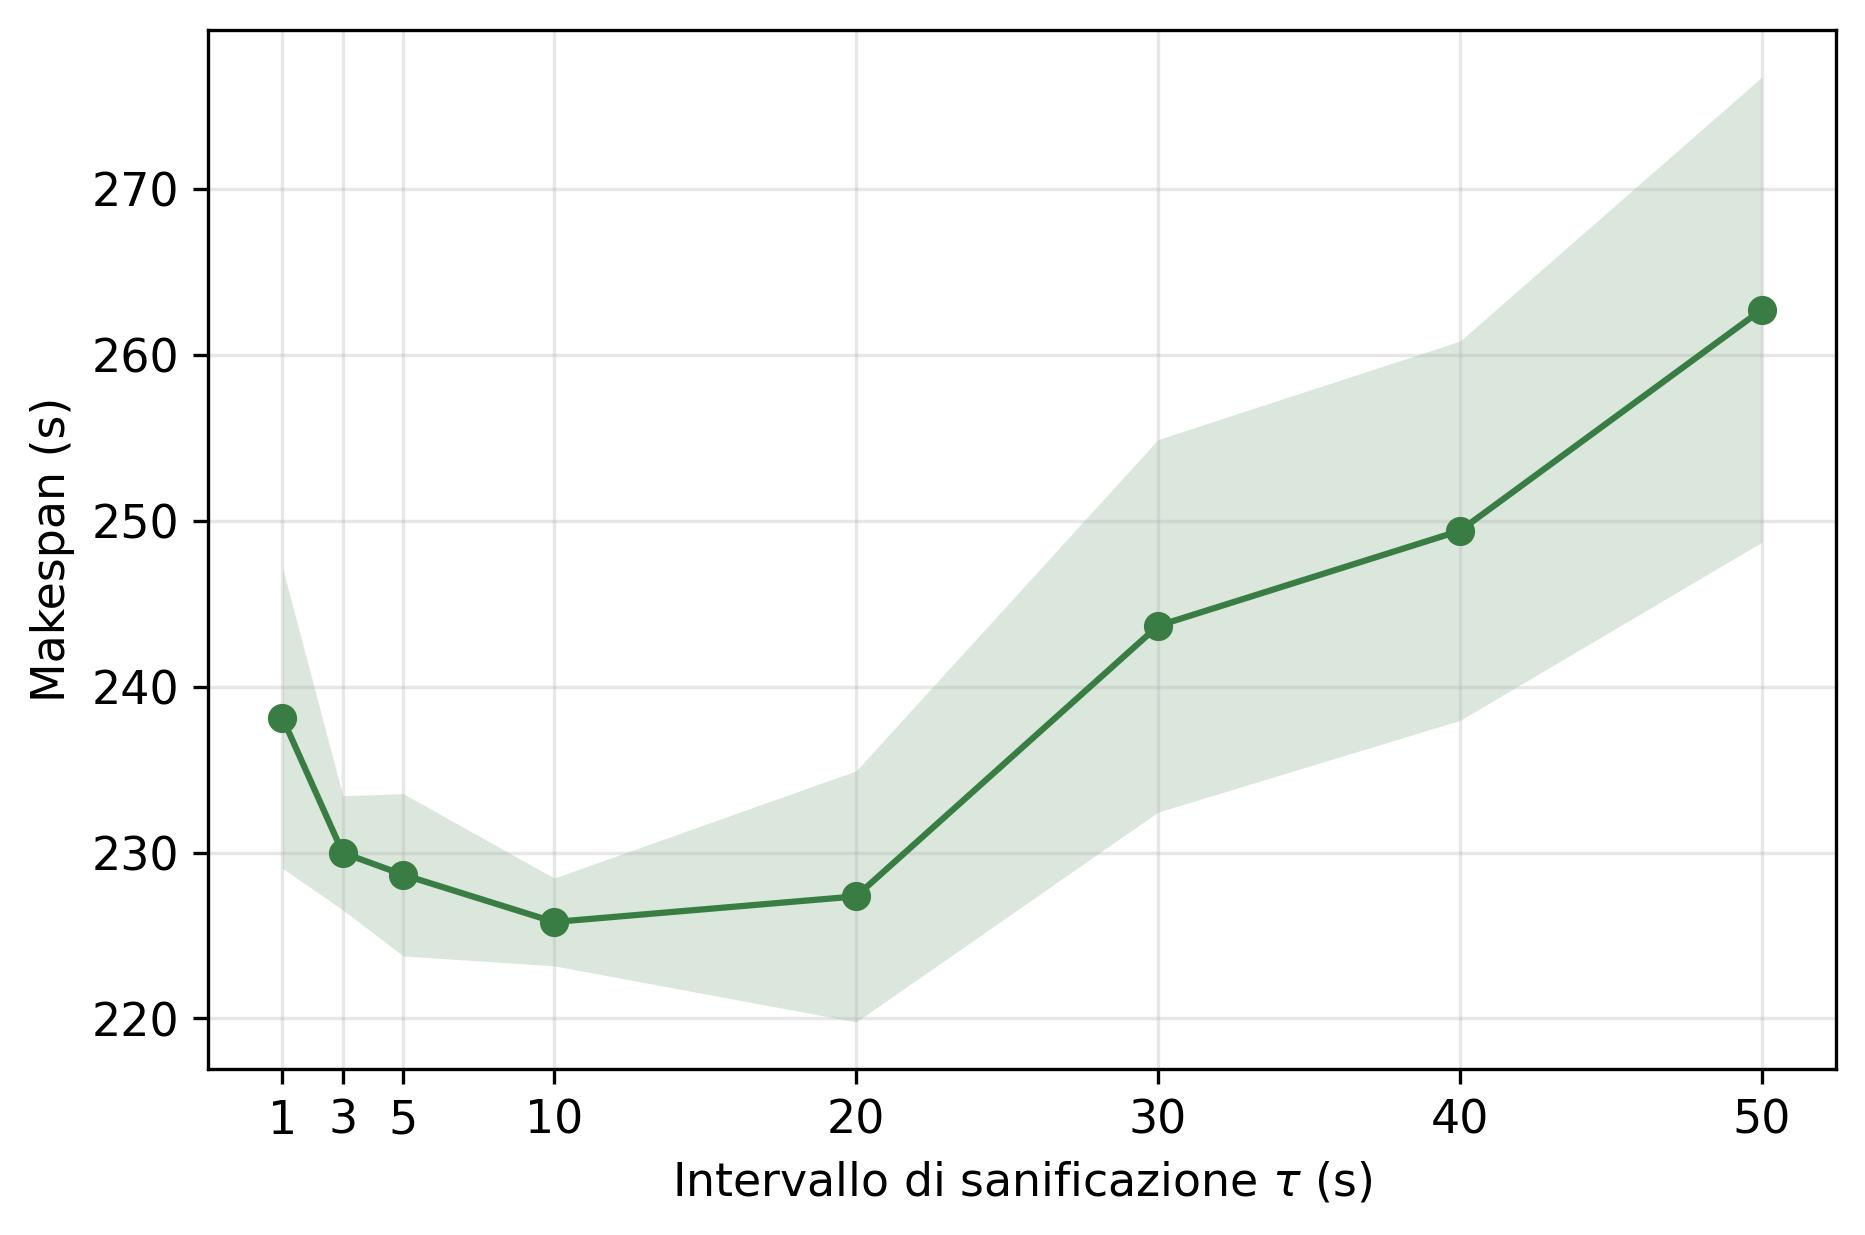
\includegraphics[width=\textwidth]{immagini/val_sanificazione/sanitize_makespan.jpg}
        \caption{Makespan del batch.}
        \label{fig:sanificazione-makespan}
    \end{subfigure}
    \caption{Costo globale della sanificazione al variare dell'intervallo $\tau$.}
    \label{fig:sanificazione-attesa-makespan}
\end{figure}

Il costo globale in termini di tempo è mostrato dalla Figura~\ref{fig:sanificazione-attesa-makespan}. L'attesa media dei task bloccati resta sui 10 secondi fino al minimo della U, per poi crescere rapidamente fino a quasi 40 secondi a $\tau = 50$. Questo chiarisce la natura asimmetrica dei due bracci: a sinistra i task vengono bloccati spesso, ma per poco tempo ciascuno, perché un nodo tornerà presto disponibile; a destra vengono bloccati meno spesso, ma chi resta bloccato attende molto più a lungo, dato che lo sblocco dipende da un ciclo di sanificazione sempre più raro. Il makespan segue anch'esso un andamento a U, molto più contenuto, con un minimo intorno ai 226 secondi nella regione ottimale e una risalita fino a circa 238 secondi a $\tau = 1$ e 263 secondi a $\tau = 50$. Anche qui la vista per batch attenua l'effetto rispetto a quella per singolo task, per via dei 200 secondi di sottomissione e della sovrapposizione delle attese, ma conferma che la regione tra 10 e 20 secondi minimizza il costo sia per il singolo task sia per il carico complessivo.

Per concludere, l'esperimento conferma l'andamento a U atteso e individua una regione ottimale dell'intervallo di sanificazione tra 10 e 20 secondi per questo carico, in cui si bilanciano i due effetti opposti. Al di sotto di questa regione la sanificazione tiene i nodi troppo spesso indisponibili, al di sopra lascia le tracce troppo a lungo sui nodi, e in entrambi i casi la latenza di scheduling peggiora.

% ------------------------------------------------------------ %

\section{Discussione e Limitazioni}
\label{sec:discussione_limitazioni}

I due esperimenti, visti insieme, misurano lo stesso compromesso di fondo anticipato all'inizio del capitolo, quello tra la disponibilità dei nodi e la reattività dello scheduling, sul quale la densità di conflitto e l'intervallo di sanificazione agiscono su lati distinti. Il primo esperimento mostra che il peso di questo compromesso cresce con il grado di conflitto, poiché più i contesti sono in conflitto tra loro più task restano bloccati in attesa che la sanificazione liberi un nodo, mentre il secondo mostra come l'intervallo di sanificazione governi il modo in cui tale attesa viene pagata, con una regione ottimale di $\tau$ in cui i nodi non sono sanificati così spesso da risultare quasi sempre indisponibili, né così di rado da restare a lungo contaminati. I due risultati si completano, dato che la densità stabilisce quanto il sistema sia esposto al blocco e la sanificazione quanto rapidamente possa liberarsene, e insieme indicano che il costo di $c_{wall}$ non è una proprietà fissa del modello ma dipende tanto dal carico sottomesso quanto dalla cadenza con cui i nodi vengono ripuliti.

Da questa lettura emerge un limite non del modello ma della strategia di sanificazione adottata, e i dati raccolti ne motivano un miglioramento in più direzioni. La sanificazione periodica, l'unica implementata nel prototipo tra quelle discusse nella Sezione~\ref{subsec:chinese_wall}, agisce a cadenza fissa e indipendentemente dallo stato dei nodi, perciò la regione ottimale individuata non è un valore universale ma dipende dal carico, collocandosi in questo caso intorno alla durata dei task, e un intervallo calibrato per un carico risulterebbe inadeguato per un altro. Una prima direzione di miglioramento sono proprio le strategie alternative già discusse nel modello, dove si osservava anche come più strategie possano essere combinate tra loro. Al posto della sola sanificazione periodica si potrebbe ad esempio adottare una combinazione di quella opportunistica e di quella basata su \emph{threshold}: la prima, intervenendo su un nodo appena questo è libero dai task attivi, mitigherebbe il braccio sinistro della curva osservata, mentre la seconda, avviando la pulizia quando la cardinalità di $\Lambda(n)$ supera una certa soglia, eviterebbe che un nodo accumuli troppi contesti e si avvicini alla saturazione.

Una seconda direzione, più sostanziale, riguarda il modo stesso in cui la sanificazione tratta il nodo e i task in esecuzione su di esso. Come descritto nella Sezione~\ref{subsec:chinese_wall}, la procedura attuale porta il nodo fuori da $\mathcal{N}$ e attende il completamento di tutti i task attivi prima di ripulirne le tracce, per cui un singolo task di lunga durata tiene il nodo indisponibile per tutti gli altri task per l'intero tempo della sua esecuzione. Si potrebbe invece rendere la pulizia parziale, lasciando il nodo in $\mathcal{N}$ e intervenendo in modo diverso sui task in base a quanto manca al loro completamento. All'avvio della sanificazione si attenderebbero soltanto i task la cui durata residua, stimata, resta sotto una certa soglia, ripulendo la loro traccia contestuale insieme a quella dei task già terminati in precedenza. I task che invece supererebbero quella soglia non verrebbero attesi, e la loro traccia resterebbe sul nodo, continuando a bloccare i soli task in conflitto con essi. In questo modo il nodo si libera di tutta la contaminazione eliminabile in tempi brevi, senza dover restare indisponibile in attesa dei pochi task più lunghi. Questo approccio però richiede di poter stimare la durata di un task, informazione che il modello attuale non possiede trattando i task come \emph{black-box}. Disporre di una stima, ricavata ad esempio dalla semantica del task, è proprio ciò che permetterebbe di decidere caso per caso se attendere il completamento di un task e ripulirne la traccia, oppure, quando la sua durata supera la soglia, procedere senza attenderlo lasciandone la traccia sul nodo. Lasciando sul nodo task ancora attivi, questa variante andrebbe accompagnata dall'estensione indicata nella Sezione~\ref{subsec:chinese_wall}, che tiene conto anche delle autorizzazioni dei rispettivi issuer.

Per finire, gli esperimenti hanno confermato le aspettative formulate senza produrre comportamenti inattesi, il che costituisce anche una verifica indiretta della correttezza del prototipo rispetto al modello teorico, ma restano alcune limitazioni, in parte già anticipate, che delimitano la portata dei risultati. La prima, discussa nella Sezione~\ref{subsec:perimetro_valutazione}, riguarda le risorse computazionali dei nodi, dato che i task, non occupando significativamente CPU o memoria, non saturano mai i nodi, mentre in un carico reale la loro saturazione costituirebbe un ulteriore fattore di ritardo, estraneo però alle politiche del modello. Una seconda deriva dall'ambiente a singola macchina descritto nella Sezione~\ref{sec:configurazione_sperimentale}, in cui tutte le componenti del cluster condividono le stesse risorse e sotto carico possono quindi introdurre leggeri ritardi non imputabili al sistema in valutazione, per cui i valori assoluti di latenza non vanno intesi come rappresentativi di un cluster di produzione reale. Infine, agli intervalli di sanificazione più lunghi una run copre pochi cicli di pulizia e la stima della latenza è dominata dalla varianza, come testimoniano le bande più ampie nella Figura~\ref{fig:sanificazione-latenza-cdf}, per cui i valori oltre l'ottimo vanno letti come tendenza più che come misure precise.